\documentclass[twoside]{book}

% Packages required by doxygen
\usepackage{fixltx2e}
\usepackage{calc}
\usepackage{doxygen}
\usepackage[export]{adjustbox} % also loads graphicx
\usepackage{graphicx}
\usepackage[utf8]{inputenc}
\usepackage{makeidx}
\usepackage{multicol}
\usepackage{multirow}
\PassOptionsToPackage{warn}{textcomp}
\usepackage{textcomp}
\usepackage[nointegrals]{wasysym}
\usepackage[table]{xcolor}

% Font selection
\usepackage[T1]{fontenc}
\usepackage[scaled=.90]{helvet}
\usepackage{courier}
\usepackage{amssymb}
\usepackage{sectsty}
\renewcommand{\familydefault}{\sfdefault}
\allsectionsfont{%
  \fontseries{bc}\selectfont%
  \color{darkgray}%
}
\renewcommand{\DoxyLabelFont}{%
  \fontseries{bc}\selectfont%
  \color{darkgray}%
}
\newcommand{\+}{\discretionary{\mbox{\scriptsize$\hookleftarrow$}}{}{}}

% Page & text layout
\usepackage{geometry}
\geometry{%
  a4paper,%
  top=2.5cm,%
  bottom=2.5cm,%
  left=2.5cm,%
  right=2.5cm%
}
\tolerance=750
\hfuzz=15pt
\hbadness=750
\setlength{\emergencystretch}{15pt}
\setlength{\parindent}{0cm}
\setlength{\parskip}{3ex plus 2ex minus 2ex}
\makeatletter
\renewcommand{\paragraph}{%
  \@startsection{paragraph}{4}{0ex}{-1.0ex}{1.0ex}{%
    \normalfont\normalsize\bfseries\SS@parafont%
  }%
}
\renewcommand{\subparagraph}{%
  \@startsection{subparagraph}{5}{0ex}{-1.0ex}{1.0ex}{%
    \normalfont\normalsize\bfseries\SS@subparafont%
  }%
}
\makeatother

% Headers & footers
\usepackage{fancyhdr}
\pagestyle{fancyplain}
\fancyhead[LE]{\fancyplain{}{\bfseries\thepage}}
\fancyhead[CE]{\fancyplain{}{}}
\fancyhead[RE]{\fancyplain{}{\bfseries\leftmark}}
\fancyhead[LO]{\fancyplain{}{\bfseries\rightmark}}
\fancyhead[CO]{\fancyplain{}{}}
\fancyhead[RO]{\fancyplain{}{\bfseries\thepage}}
\fancyfoot[LE]{\fancyplain{}{}}
\fancyfoot[CE]{\fancyplain{}{}}
\fancyfoot[RE]{\fancyplain{}{\bfseries\scriptsize Generated by Doxygen }}
\fancyfoot[LO]{\fancyplain{}{\bfseries\scriptsize Generated by Doxygen }}
\fancyfoot[CO]{\fancyplain{}{}}
\fancyfoot[RO]{\fancyplain{}{}}
\renewcommand{\footrulewidth}{0.4pt}
\renewcommand{\chaptermark}[1]{%
  \markboth{#1}{}%
}
\renewcommand{\sectionmark}[1]{%
  \markright{\thesection\ #1}%
}

% Indices & bibliography
\usepackage{natbib}
\usepackage[titles]{tocloft}
\setcounter{tocdepth}{3}
\setcounter{secnumdepth}{5}
\makeindex

% Hyperlinks (required, but should be loaded last)
\usepackage{ifpdf}
\ifpdf
  \usepackage[pdftex,pagebackref=true]{hyperref}
\else
  \usepackage[ps2pdf,pagebackref=true]{hyperref}
\fi
\hypersetup{%
  colorlinks=true,%
  linkcolor=blue,%
  citecolor=blue,%
  unicode%
}

% Custom commands
\newcommand{\clearemptydoublepage}{%
  \newpage{\pagestyle{empty}\cleardoublepage}%
}

\usepackage{caption}
\captionsetup{labelsep=space,justification=centering,font={bf},singlelinecheck=off,skip=4pt,position=top}

%===== C O N T E N T S =====

\begin{document}

% Titlepage & ToC
\hypersetup{pageanchor=false,
             bookmarksnumbered=true,
             pdfencoding=unicode
            }
\pagenumbering{alph}
\begin{titlepage}
\vspace*{7cm}
\begin{center}%
{\Large S\+GL -\/ Simple Graphing Library }\\
\vspace*{1cm}
{\large Generated by Doxygen 1.8.14}\\
\end{center}
\end{titlepage}
\clearemptydoublepage
\pagenumbering{roman}
\tableofcontents
\clearemptydoublepage
\pagenumbering{arabic}
\hypersetup{pageanchor=true}

%--- Begin generated contents ---
\chapter{Namespace Index}
\section{Namespace List}
Here is a list of all documented namespaces with brief descriptions\+:\begin{DoxyCompactList}
\item\contentsline{section}{\mbox{\hyperlink{namespace_s_g_l}{S\+GL}} }{\pageref{namespace_s_g_l}}{}
\end{DoxyCompactList}

\chapter{Hierarchical Index}
\section{Class Hierarchy}
This inheritance list is sorted roughly, but not completely, alphabetically\+:\begin{DoxyCompactList}
\item \contentsline{section}{S\+G\+L.\+Graph}{\pageref{class_s_g_l_1_1_graph}}{}
\item I\+Equatable\begin{DoxyCompactList}
\item \contentsline{section}{S\+G\+L.\+Ellipse}{\pageref{class_s_g_l_1_1_ellipse}}{}
\item \contentsline{section}{S\+G\+L.\+Label}{\pageref{class_s_g_l_1_1_label}}{}
\item \contentsline{section}{S\+G\+L.\+Line}{\pageref{class_s_g_l_1_1_line}}{}
\item \contentsline{section}{S\+G\+L.\+Point}{\pageref{struct_s_g_l_1_1_point}}{}
\item \contentsline{section}{S\+G\+L.\+Rectangle}{\pageref{class_s_g_l_1_1_rectangle}}{}
\end{DoxyCompactList}
\end{DoxyCompactList}

\chapter{Class Index}
\section{Class List}
Here are the classes, structs, unions and interfaces with brief descriptions\+:\begin{DoxyCompactList}
\item\contentsline{section}{\mbox{\hyperlink{class_s_g_l_1_1_ellipse}{S\+G\+L.\+Ellipse}} \\*Represent an ellipse defined by an origin point and two radii (along the X and Y axes). }{\pageref{class_s_g_l_1_1_ellipse}}{}
\item\contentsline{section}{\mbox{\hyperlink{class_s_g_l_1_1_graph}{S\+G\+L.\+Graph}} \\*A graphical chart that is shown in a separate window. }{\pageref{class_s_g_l_1_1_graph}}{}
\item\contentsline{section}{\mbox{\hyperlink{class_s_g_l_1_1_label}{S\+G\+L.\+Label}} \\*Represent some text on the graph, defined by an origin point and a text message. }{\pageref{class_s_g_l_1_1_label}}{}
\item\contentsline{section}{\mbox{\hyperlink{class_s_g_l_1_1_line}{S\+G\+L.\+Line}} \\*Represent a line defined by two points. }{\pageref{class_s_g_l_1_1_line}}{}
\item\contentsline{section}{\mbox{\hyperlink{struct_s_g_l_1_1_point}{S\+G\+L.\+Point}} \\*Represent a point defined by two coordinates (X and Y). }{\pageref{struct_s_g_l_1_1_point}}{}
\item\contentsline{section}{\mbox{\hyperlink{class_s_g_l_1_1_rectangle}{S\+G\+L.\+Rectangle}} \\*Represent a rectangle defined by its center and side dimensions. }{\pageref{class_s_g_l_1_1_rectangle}}{}
\end{DoxyCompactList}

\chapter{Namespace Documentation}
\hypertarget{namespace_s_g_l}{}\section{S\+GL Namespace Reference}
\label{namespace_s_g_l}\index{S\+GL@{S\+GL}}
\subsection*{Classes}
\begin{DoxyCompactItemize}
\item 
class \mbox{\hyperlink{class_s_g_l_1_1_ellipse}{Ellipse}}
\begin{DoxyCompactList}\small\item\em Represent an ellipse defined by an origin point and two radii (along the X and Y axes). \end{DoxyCompactList}\item 
class \mbox{\hyperlink{class_s_g_l_1_1_graph}{Graph}}
\begin{DoxyCompactList}\small\item\em A graphical chart that is shown in a separate window. \end{DoxyCompactList}\item 
class \mbox{\hyperlink{class_s_g_l_1_1_label}{Label}}
\begin{DoxyCompactList}\small\item\em Represent some text on the graph, defined by an origin point and a text message. \end{DoxyCompactList}\item 
class \mbox{\hyperlink{class_s_g_l_1_1_line}{Line}}
\begin{DoxyCompactList}\small\item\em Represent a line defined by two points. \end{DoxyCompactList}\item 
struct \mbox{\hyperlink{struct_s_g_l_1_1_point}{Point}}
\begin{DoxyCompactList}\small\item\em Represent a point defined by two coordinates (X and Y). \end{DoxyCompactList}\item 
class \mbox{\hyperlink{class_s_g_l_1_1_rectangle}{Rectangle}}
\begin{DoxyCompactList}\small\item\em Represent a rectangle defined by its center and side dimensions. \end{DoxyCompactList}\item 
class {\bfseries Utils}
\begin{DoxyCompactList}\small\item\em A static class containing some utility methods. \end{DoxyCompactList}\end{DoxyCompactItemize}
\subsection*{Enumerations}
\begin{DoxyCompactItemize}
\item 
enum \mbox{\hyperlink{namespace_s_g_l_aa8de446c655c151ef21cfe27b24da87c}{Alignment}} \{ \newline
{\bfseries Center}, 
{\bfseries Top}, 
{\bfseries Left}, 
{\bfseries Right}, 
\newline
{\bfseries Bottom}
 \}
\begin{DoxyCompactList}\small\item\em Represents the position of the label relative the point. \end{DoxyCompactList}\end{DoxyCompactItemize}


\subsection{Enumeration Type Documentation}
\mbox{\Hypertarget{namespace_s_g_l_aa8de446c655c151ef21cfe27b24da87c}\label{namespace_s_g_l_aa8de446c655c151ef21cfe27b24da87c}} 
\index{S\+GL@{S\+GL}!Alignment@{Alignment}}
\index{Alignment@{Alignment}!S\+GL@{S\+GL}}
\subsubsection{\texorpdfstring{Alignment}{Alignment}}
{\footnotesize\ttfamily enum \mbox{\hyperlink{namespace_s_g_l_aa8de446c655c151ef21cfe27b24da87c}{S\+G\+L.\+Alignment}}\hspace{0.3cm}{\ttfamily [strong]}}



Represents the position of the label relative the point. 


\chapter{Class Documentation}
\hypertarget{class_s_g_l_1_1_ellipse}{}\section{S\+G\+L.\+Ellipse Class Reference}
\label{class_s_g_l_1_1_ellipse}\index{S\+G\+L.\+Ellipse@{S\+G\+L.\+Ellipse}}


Represent an ellipse defined by an origin point and two radii (along the X and Y axes).  


Inheritance diagram for S\+G\+L.\+Ellipse\+:\begin{figure}[H]
\begin{center}
\leavevmode
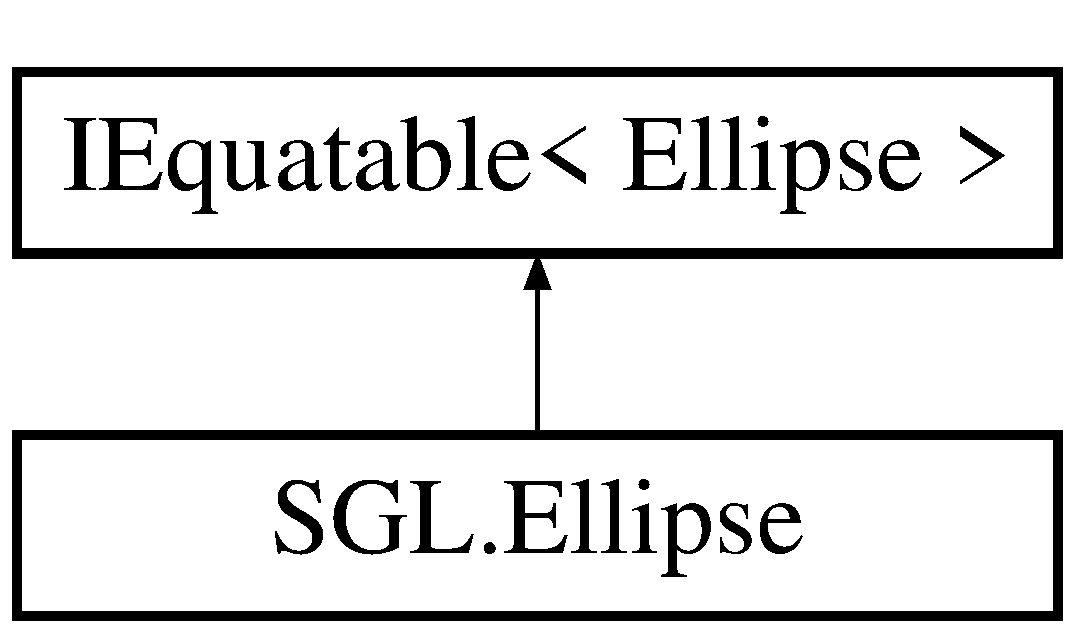
\includegraphics[height=2.000000cm]{class_s_g_l_1_1_ellipse}
\end{center}
\end{figure}
\subsection*{Public Member Functions}
\begin{DoxyCompactItemize}
\item 
\mbox{\Hypertarget{class_s_g_l_1_1_ellipse_ab7c43658b938824f2f89241e5d2a1a3e}\label{class_s_g_l_1_1_ellipse_ab7c43658b938824f2f89241e5d2a1a3e}} 
{\bfseries Ellipse} (double x, double y, double rx, double ry)
\item 
\mbox{\Hypertarget{class_s_g_l_1_1_ellipse_a7e84a523ff15e2de67f636bc8f832594}\label{class_s_g_l_1_1_ellipse_a7e84a523ff15e2de67f636bc8f832594}} 
{\bfseries Ellipse} (double x, double y, double radius)
\item 
\mbox{\Hypertarget{class_s_g_l_1_1_ellipse_ab4aaaa32ad5f69a406fd31cce901b0af}\label{class_s_g_l_1_1_ellipse_ab4aaaa32ad5f69a406fd31cce901b0af}} 
{\bfseries Ellipse} (\mbox{\hyperlink{struct_s_g_l_1_1_point}{Point}} p, double width, double height)
\item 
\mbox{\Hypertarget{class_s_g_l_1_1_ellipse_a62eb72ea81594ca6e2449466493d6204}\label{class_s_g_l_1_1_ellipse_a62eb72ea81594ca6e2449466493d6204}} 
{\bfseries Ellipse} (\mbox{\hyperlink{struct_s_g_l_1_1_point}{Point}} p, double radius)
\item 
bool \mbox{\hyperlink{class_s_g_l_1_1_ellipse_a4aa98efe82607feabecf228d21339e00}{Contains}} (\mbox{\hyperlink{struct_s_g_l_1_1_point}{Point}} p)
\begin{DoxyCompactList}\small\item\em Checks whether the ellipse contains the point. \end{DoxyCompactList}\item 
\mbox{\Hypertarget{class_s_g_l_1_1_ellipse_a9357f80bbe482175b1a7c6e4ece54456}\label{class_s_g_l_1_1_ellipse_a9357f80bbe482175b1a7c6e4ece54456}} 
bool {\bfseries Equals} (\mbox{\hyperlink{class_s_g_l_1_1_ellipse}{Ellipse}} other)
\item 
\mbox{\Hypertarget{class_s_g_l_1_1_ellipse_ad54b2bf09ec36069e1826535d0fc363a}\label{class_s_g_l_1_1_ellipse_ad54b2bf09ec36069e1826535d0fc363a}} 
override bool {\bfseries Equals} (object obj)
\item 
\mbox{\Hypertarget{class_s_g_l_1_1_ellipse_aa04cd2fefc7a4a920406af242025eb6d}\label{class_s_g_l_1_1_ellipse_aa04cd2fefc7a4a920406af242025eb6d}} 
override int {\bfseries Get\+Hash\+Code} ()
\item 
\mbox{\Hypertarget{class_s_g_l_1_1_ellipse_ae24cbc23530de4b3dd1ac46b79216864}\label{class_s_g_l_1_1_ellipse_ae24cbc23530de4b3dd1ac46b79216864}} 
override string {\bfseries To\+String} ()
\end{DoxyCompactItemize}
\subsection*{Static Public Member Functions}
\begin{DoxyCompactItemize}
\item 
\mbox{\Hypertarget{class_s_g_l_1_1_ellipse_a972329f722dcc91f3f56fb8906ee1177}\label{class_s_g_l_1_1_ellipse_a972329f722dcc91f3f56fb8906ee1177}} 
static bool {\bfseries operator==} (\mbox{\hyperlink{class_s_g_l_1_1_ellipse}{Ellipse}} a, \mbox{\hyperlink{class_s_g_l_1_1_ellipse}{Ellipse}} b)
\item 
\mbox{\Hypertarget{class_s_g_l_1_1_ellipse_af5e66ec61f3fbbd363bbd3cf52482841}\label{class_s_g_l_1_1_ellipse_af5e66ec61f3fbbd363bbd3cf52482841}} 
static bool {\bfseries operator!=} (\mbox{\hyperlink{class_s_g_l_1_1_ellipse}{Ellipse}} a, \mbox{\hyperlink{class_s_g_l_1_1_ellipse}{Ellipse}} b)
\end{DoxyCompactItemize}
\subsection*{Public Attributes}
\begin{DoxyCompactItemize}
\item 
double \mbox{\hyperlink{class_s_g_l_1_1_ellipse_a8259d2766fa4d206859cdc874100517b}{Area}} =$>$ Math.\+PI $\ast$ \mbox{\hyperlink{class_s_g_l_1_1_ellipse_ac6630cfb928ba11742a1efefe7ed41ca}{RX}} $\ast$ \mbox{\hyperlink{class_s_g_l_1_1_ellipse_af1df83b66e02fb6ebf969e608fc018d9}{RY}}
\begin{DoxyCompactList}\small\item\em The area of the ellipse. \end{DoxyCompactList}\item 
double \mbox{\hyperlink{class_s_g_l_1_1_ellipse_a3f9ecf8407c0b189ca037c4d51306786}{Perimeter}} =$>$ \mbox{\hyperlink{class_s_g_l_1_1_ellipse_ac8c377f7d5e0efb4ca338e67fede6450}{Circumference}}
\begin{DoxyCompactList}\small\item\em The outer perimeter of the ellipse. Synonymous with \mbox{\hyperlink{class_s_g_l_1_1_ellipse_ac8c377f7d5e0efb4ca338e67fede6450}{Circumference}}. \end{DoxyCompactList}\end{DoxyCompactItemize}
\subsection*{Properties}
\begin{DoxyCompactItemize}
\item 
\mbox{\hyperlink{struct_s_g_l_1_1_point}{Point}} \mbox{\hyperlink{class_s_g_l_1_1_ellipse_a0f9ae80639bd70e68bed0513e8fe91bb}{Center}}\hspace{0.3cm}{\ttfamily  \mbox{[}get, set\mbox{]}}
\begin{DoxyCompactList}\small\item\em The center of the ellipse. \end{DoxyCompactList}\item 
double \mbox{\hyperlink{class_s_g_l_1_1_ellipse_a79ef810cf7ed8d3911da64df3c846869}{X}}\hspace{0.3cm}{\ttfamily  \mbox{[}get, set\mbox{]}}
\begin{DoxyCompactList}\small\item\em The X-\/coordinate of the center of the ellipse. \end{DoxyCompactList}\item 
double \mbox{\hyperlink{class_s_g_l_1_1_ellipse_a50e30bc042f57afbdf34924a0435fc21}{Y}}\hspace{0.3cm}{\ttfamily  \mbox{[}get, set\mbox{]}}
\begin{DoxyCompactList}\small\item\em The Y-\/coordinate of the center of the ellipse. \end{DoxyCompactList}\item 
double \mbox{\hyperlink{class_s_g_l_1_1_ellipse_ac6630cfb928ba11742a1efefe7ed41ca}{RX}}\hspace{0.3cm}{\ttfamily  \mbox{[}get, set\mbox{]}}
\begin{DoxyCompactList}\small\item\em The radius along the X-\/axis. \end{DoxyCompactList}\item 
double \mbox{\hyperlink{class_s_g_l_1_1_ellipse_af1df83b66e02fb6ebf969e608fc018d9}{RY}}\hspace{0.3cm}{\ttfamily  \mbox{[}get, set\mbox{]}}
\begin{DoxyCompactList}\small\item\em The radius along the Y-\/axis. \end{DoxyCompactList}\item 
double \mbox{\hyperlink{class_s_g_l_1_1_ellipse_ac8c377f7d5e0efb4ca338e67fede6450}{Circumference}}\hspace{0.3cm}{\ttfamily  \mbox{[}get\mbox{]}}
\begin{DoxyCompactList}\small\item\em The outer perimeter of the ellipse. \end{DoxyCompactList}\end{DoxyCompactItemize}


\subsection{Detailed Description}
Represent an ellipse defined by an origin point and two radii (along the X and Y axes). 



\subsection{Member Function Documentation}
\mbox{\Hypertarget{class_s_g_l_1_1_ellipse_a4aa98efe82607feabecf228d21339e00}\label{class_s_g_l_1_1_ellipse_a4aa98efe82607feabecf228d21339e00}} 
\index{S\+G\+L\+::\+Ellipse@{S\+G\+L\+::\+Ellipse}!Contains@{Contains}}
\index{Contains@{Contains}!S\+G\+L\+::\+Ellipse@{S\+G\+L\+::\+Ellipse}}
\subsubsection{\texorpdfstring{Contains()}{Contains()}}
{\footnotesize\ttfamily bool S\+G\+L.\+Ellipse.\+Contains (\begin{DoxyParamCaption}\item[{\mbox{\hyperlink{struct_s_g_l_1_1_point}{Point}}}]{p }\end{DoxyParamCaption})\hspace{0.3cm}{\ttfamily [inline]}}



Checks whether the ellipse contains the point. 



\subsection{Member Data Documentation}
\mbox{\Hypertarget{class_s_g_l_1_1_ellipse_a8259d2766fa4d206859cdc874100517b}\label{class_s_g_l_1_1_ellipse_a8259d2766fa4d206859cdc874100517b}} 
\index{S\+G\+L\+::\+Ellipse@{S\+G\+L\+::\+Ellipse}!Area@{Area}}
\index{Area@{Area}!S\+G\+L\+::\+Ellipse@{S\+G\+L\+::\+Ellipse}}
\subsubsection{\texorpdfstring{Area}{Area}}
{\footnotesize\ttfamily double S\+G\+L.\+Ellipse.\+Area =$>$ Math.\+PI $\ast$ \mbox{\hyperlink{class_s_g_l_1_1_ellipse_ac6630cfb928ba11742a1efefe7ed41ca}{RX}} $\ast$ \mbox{\hyperlink{class_s_g_l_1_1_ellipse_af1df83b66e02fb6ebf969e608fc018d9}{RY}}}



The area of the ellipse. 

\mbox{\Hypertarget{class_s_g_l_1_1_ellipse_a3f9ecf8407c0b189ca037c4d51306786}\label{class_s_g_l_1_1_ellipse_a3f9ecf8407c0b189ca037c4d51306786}} 
\index{S\+G\+L\+::\+Ellipse@{S\+G\+L\+::\+Ellipse}!Perimeter@{Perimeter}}
\index{Perimeter@{Perimeter}!S\+G\+L\+::\+Ellipse@{S\+G\+L\+::\+Ellipse}}
\subsubsection{\texorpdfstring{Perimeter}{Perimeter}}
{\footnotesize\ttfamily double S\+G\+L.\+Ellipse.\+Perimeter =$>$ \mbox{\hyperlink{class_s_g_l_1_1_ellipse_ac8c377f7d5e0efb4ca338e67fede6450}{Circumference}}}



The outer perimeter of the ellipse. Synonymous with \mbox{\hyperlink{class_s_g_l_1_1_ellipse_ac8c377f7d5e0efb4ca338e67fede6450}{Circumference}}. 



\subsection{Property Documentation}
\mbox{\Hypertarget{class_s_g_l_1_1_ellipse_a0f9ae80639bd70e68bed0513e8fe91bb}\label{class_s_g_l_1_1_ellipse_a0f9ae80639bd70e68bed0513e8fe91bb}} 
\index{S\+G\+L\+::\+Ellipse@{S\+G\+L\+::\+Ellipse}!Center@{Center}}
\index{Center@{Center}!S\+G\+L\+::\+Ellipse@{S\+G\+L\+::\+Ellipse}}
\subsubsection{\texorpdfstring{Center}{Center}}
{\footnotesize\ttfamily \mbox{\hyperlink{struct_s_g_l_1_1_point}{Point}} S\+G\+L.\+Ellipse.\+Center\hspace{0.3cm}{\ttfamily [get]}, {\ttfamily [set]}}



The center of the ellipse. 

\mbox{\Hypertarget{class_s_g_l_1_1_ellipse_ac8c377f7d5e0efb4ca338e67fede6450}\label{class_s_g_l_1_1_ellipse_ac8c377f7d5e0efb4ca338e67fede6450}} 
\index{S\+G\+L\+::\+Ellipse@{S\+G\+L\+::\+Ellipse}!Circumference@{Circumference}}
\index{Circumference@{Circumference}!S\+G\+L\+::\+Ellipse@{S\+G\+L\+::\+Ellipse}}
\subsubsection{\texorpdfstring{Circumference}{Circumference}}
{\footnotesize\ttfamily double S\+G\+L.\+Ellipse.\+Circumference\hspace{0.3cm}{\ttfamily [get]}}



The outer perimeter of the ellipse. 

\mbox{\Hypertarget{class_s_g_l_1_1_ellipse_ac6630cfb928ba11742a1efefe7ed41ca}\label{class_s_g_l_1_1_ellipse_ac6630cfb928ba11742a1efefe7ed41ca}} 
\index{S\+G\+L\+::\+Ellipse@{S\+G\+L\+::\+Ellipse}!RX@{RX}}
\index{RX@{RX}!S\+G\+L\+::\+Ellipse@{S\+G\+L\+::\+Ellipse}}
\subsubsection{\texorpdfstring{RX}{RX}}
{\footnotesize\ttfamily double S\+G\+L.\+Ellipse.\+RX\hspace{0.3cm}{\ttfamily [get]}, {\ttfamily [set]}}



The radius along the X-\/axis. 

\mbox{\Hypertarget{class_s_g_l_1_1_ellipse_af1df83b66e02fb6ebf969e608fc018d9}\label{class_s_g_l_1_1_ellipse_af1df83b66e02fb6ebf969e608fc018d9}} 
\index{S\+G\+L\+::\+Ellipse@{S\+G\+L\+::\+Ellipse}!RY@{RY}}
\index{RY@{RY}!S\+G\+L\+::\+Ellipse@{S\+G\+L\+::\+Ellipse}}
\subsubsection{\texorpdfstring{RY}{RY}}
{\footnotesize\ttfamily double S\+G\+L.\+Ellipse.\+RY\hspace{0.3cm}{\ttfamily [get]}, {\ttfamily [set]}}



The radius along the Y-\/axis. 

\mbox{\Hypertarget{class_s_g_l_1_1_ellipse_a79ef810cf7ed8d3911da64df3c846869}\label{class_s_g_l_1_1_ellipse_a79ef810cf7ed8d3911da64df3c846869}} 
\index{S\+G\+L\+::\+Ellipse@{S\+G\+L\+::\+Ellipse}!X@{X}}
\index{X@{X}!S\+G\+L\+::\+Ellipse@{S\+G\+L\+::\+Ellipse}}
\subsubsection{\texorpdfstring{X}{X}}
{\footnotesize\ttfamily double S\+G\+L.\+Ellipse.\+X\hspace{0.3cm}{\ttfamily [get]}, {\ttfamily [set]}}



The X-\/coordinate of the center of the ellipse. 

\mbox{\Hypertarget{class_s_g_l_1_1_ellipse_a50e30bc042f57afbdf34924a0435fc21}\label{class_s_g_l_1_1_ellipse_a50e30bc042f57afbdf34924a0435fc21}} 
\index{S\+G\+L\+::\+Ellipse@{S\+G\+L\+::\+Ellipse}!Y@{Y}}
\index{Y@{Y}!S\+G\+L\+::\+Ellipse@{S\+G\+L\+::\+Ellipse}}
\subsubsection{\texorpdfstring{Y}{Y}}
{\footnotesize\ttfamily double S\+G\+L.\+Ellipse.\+Y\hspace{0.3cm}{\ttfamily [get]}, {\ttfamily [set]}}



The Y-\/coordinate of the center of the ellipse. 



The documentation for this class was generated from the following file\+:\begin{DoxyCompactItemize}
\item 
Ellipse.\+cs\end{DoxyCompactItemize}

\hypertarget{class_s_g_l_1_1_graph}{}\section{S\+G\+L.\+Graph Class Reference}
\label{class_s_g_l_1_1_graph}\index{S\+G\+L.\+Graph@{S\+G\+L.\+Graph}}


A graphical chart that is shown in a separate window.  


\subsection*{Public Member Functions}
\begin{DoxyCompactItemize}
\item 
\mbox{\hyperlink{class_s_g_l_1_1_graph_ae49041037b01a96e44314f7b3b9b6166}{Graph}} (double range, string title=\char`\"{}Main Window\char`\"{}, double width=800, double height=640)
\begin{DoxyCompactList}\small\item\em Creates a new empty chart window. \end{DoxyCompactList}\item 
bool \mbox{\hyperlink{class_s_g_l_1_1_graph_aba994e0f4ec93be3f3d181fa128db070}{Is\+Key\+Down}} (Key key)
\begin{DoxyCompactList}\small\item\em Checks if the specified key is currently pressed. \end{DoxyCompactList}\item 
bool \mbox{\hyperlink{class_s_g_l_1_1_graph_a274ab575056c833cd3f3f45770c20b58}{Is\+Mouse\+Button\+Down}} (Mouse\+Button button)
\begin{DoxyCompactList}\small\item\em Checks if the specified mouse button is currently pressed. \end{DoxyCompactList}\item 
\mbox{\hyperlink{struct_s_g_l_1_1_point}{Point}} \mbox{\hyperlink{class_s_g_l_1_1_graph_a02daa8a4a7e540677d76e9a0ac40039d}{Select\+Point}} ()
\begin{DoxyCompactList}\small\item\em Asks the user to select a point on the chart and returns the coordinates of that point. \end{DoxyCompactList}\item 
void \mbox{\hyperlink{class_s_g_l_1_1_graph_ac67339a4d4304b41258344692535c139}{Show}} ()
\begin{DoxyCompactList}\small\item\em Shows the window. \end{DoxyCompactList}\item 
void \mbox{\hyperlink{class_s_g_l_1_1_graph_ad01766cdde14e9f9bcae84caa9d5351d}{Hide}} ()
\begin{DoxyCompactList}\small\item\em Hides the window. \end{DoxyCompactList}\item 
void \mbox{\hyperlink{class_s_g_l_1_1_graph_ab39ea13f352304658601da75c8207b08}{Close}} ()
\begin{DoxyCompactList}\small\item\em Closes the window. \end{DoxyCompactList}\item 
void \mbox{\hyperlink{class_s_g_l_1_1_graph_ad1f5ca5a92e9a3c788178e44d65ba005}{Clear}} ()
\begin{DoxyCompactList}\small\item\em Clears the content of the chart. \end{DoxyCompactList}\item 
void \mbox{\hyperlink{class_s_g_l_1_1_graph_a6b99d7fed85538b0dd5906e359fcf9c0}{Wait\+For\+Exit}} ()
\begin{DoxyCompactList}\small\item\em Waits for the user to manually close the window. \end{DoxyCompactList}\item 
int \mbox{\hyperlink{class_s_g_l_1_1_graph_a4162119a26ba960884e3660c0750d14c}{Read\+Int}} (string message=\char`\"{}Please, enter an integer.\char`\"{}, int default\+Value=0)
\begin{DoxyCompactList}\small\item\em Reads a 32-\/bit integer from the user through a graphical prompt. \end{DoxyCompactList}\item 
long \mbox{\hyperlink{class_s_g_l_1_1_graph_aa55701744ab9d06019ff60e4d2da0a16}{Read\+Long}} (string message=\char`\"{}Please, enter an integer.\char`\"{}, long default\+Value=0)
\begin{DoxyCompactList}\small\item\em Reads a 64-\/bit integer from the user through a graphical prompt. \end{DoxyCompactList}\item 
float \mbox{\hyperlink{class_s_g_l_1_1_graph_aa9d57659823175542533c9cceeeb1ff6}{Read\+Float}} (string message=\char`\"{}Please, enter a number.\char`\"{}, float default\+Value=0f)
\begin{DoxyCompactList}\small\item\em Reads a 32-\/bit floating point number from the user through a graphical prompt. \end{DoxyCompactList}\item 
double \mbox{\hyperlink{class_s_g_l_1_1_graph_ab84327403a05e999998f54b1bc4d1c35}{Read\+Double}} (string message=\char`\"{}Please, enter a number.\char`\"{}, double default\+Value=0.\+0)
\begin{DoxyCompactList}\small\item\em Reads a 64-\/bit floating point number from the user through a graphical prompt. \end{DoxyCompactList}\item 
string \mbox{\hyperlink{class_s_g_l_1_1_graph_a25db2a007fb5adaa390a44f16d4d653e}{Read\+String}} (string message=\char`\"{}Please, enter some text.\char`\"{}, string default\+Value=\char`\"{}\char`\"{})
\begin{DoxyCompactList}\small\item\em Reads a string from the user through a graphical prompt. \end{DoxyCompactList}\item 
bool \mbox{\hyperlink{class_s_g_l_1_1_graph_add2e8a9bb0b5174fc9a80e21b7d407e8}{Yes\+Or\+No}} (string message, bool default\+Value=true)
\begin{DoxyCompactList}\small\item\em Asks the user a questing and allows them to answer it with yer (true) or no (false) through a graphical prompt. \end{DoxyCompactList}\item 
T \mbox{\hyperlink{class_s_g_l_1_1_graph_a482da34c25dc49ec1fe1aed288d2807a}{Select\+Item$<$ T $>$}} (string message, T\mbox{[}$\,$\mbox{]} options, int default\+Index=-\/1)
\begin{DoxyCompactList}\small\item\em Asks the user to select an item from the list and returns the selected item. \end{DoxyCompactList}\item 
int \mbox{\hyperlink{class_s_g_l_1_1_graph_ab1d2be74da25ee0a40829993a2f597c4}{Select\+Index$<$ T $>$}} (string message, T\mbox{[}$\,$\mbox{]} options, int default\+Index=-\/1)
\begin{DoxyCompactList}\small\item\em Asks the user to select an item from the list and returns the selected item. \end{DoxyCompactList}\item 
void \mbox{\hyperlink{class_s_g_l_1_1_graph_a16bfdc1d809835f73bd9870af125b161}{Notify}} (string message)
\begin{DoxyCompactList}\small\item\em Shows a message to the user. \end{DoxyCompactList}\item 
void \mbox{\hyperlink{class_s_g_l_1_1_graph_acdd26dba75282796ec6d22b5be177b7e}{Draw}} (Func$<$ double, double $>$ f, double start=double.\+Min\+Value, double end=double.\+Max\+Value)
\begin{DoxyCompactList}\small\item\em Adds the graph of a function to the chart. The start and end of the values along the X-\/axis can also be specified. \end{DoxyCompactList}\item 
void \mbox{\hyperlink{class_s_g_l_1_1_graph_ae56a2ac44e31ab8e8dae5dc042e8515d}{Erase}} (Func$<$ double, double $>$ f, double start=double.\+Min\+Value, double end=double.\+Max\+Value)
\begin{DoxyCompactList}\small\item\em Erases a function that is currently displayed on the graph. The start and end of the values along the X-\/axis can also be specified. \end{DoxyCompactList}\item 
void \mbox{\hyperlink{class_s_g_l_1_1_graph_ab406eaa6b30080e663cd2152e8fd36d2}{Draw\+Axes}} ()
\begin{DoxyCompactList}\small\item\em Adds the X and Y axes to the graph. \end{DoxyCompactList}\item 
void \mbox{\hyperlink{class_s_g_l_1_1_graph_a5fa59d087be175868fe52c4b81f4c724}{Draw}} (\mbox{\hyperlink{class_s_g_l_1_1_label}{Label}} t)
\begin{DoxyCompactList}\small\item\em Adds a line of text to the chart. \end{DoxyCompactList}\item 
void \mbox{\hyperlink{class_s_g_l_1_1_graph_a794de8a13de541b1b6e43a94469a1801}{Erase}} (\mbox{\hyperlink{class_s_g_l_1_1_label}{Label}} t)
\begin{DoxyCompactList}\small\item\em Removes a currently visible line of text from the chart. \end{DoxyCompactList}\item 
void \mbox{\hyperlink{class_s_g_l_1_1_graph_ae4409704a5d6224c6f8a007977922bb8}{Draw}} (\mbox{\hyperlink{class_s_g_l_1_1_line}{Line}} l)
\begin{DoxyCompactList}\small\item\em Adds a line to the chart. \end{DoxyCompactList}\item 
void \mbox{\hyperlink{class_s_g_l_1_1_graph_ae091fb4ee52a500a4c6d186bc4b5d27f}{Erase}} (\mbox{\hyperlink{class_s_g_l_1_1_line}{Line}} l)
\begin{DoxyCompactList}\small\item\em Removes a currently visible line from the chart. \end{DoxyCompactList}\item 
void \mbox{\hyperlink{class_s_g_l_1_1_graph_ab9f18f59b4f05c9a3dcb2277634532d5}{Draw}} (\mbox{\hyperlink{class_s_g_l_1_1_rectangle}{Rectangle}} r)
\begin{DoxyCompactList}\small\item\em Adds a rectangle to the chart. \end{DoxyCompactList}\item 
void \mbox{\hyperlink{class_s_g_l_1_1_graph_ae0b009d2b01edfb52598f28fc89728da}{Erase}} (\mbox{\hyperlink{class_s_g_l_1_1_rectangle}{Rectangle}} r)
\begin{DoxyCompactList}\small\item\em Removes a currently visible rectangle from the chart. \end{DoxyCompactList}\item 
void \mbox{\hyperlink{class_s_g_l_1_1_graph_a2ef792871c730c14e38d7b33e97b7540}{Draw}} (\mbox{\hyperlink{struct_s_g_l_1_1_point}{Point}} p)
\begin{DoxyCompactList}\small\item\em Adds a point to the chart. \end{DoxyCompactList}\item 
void \mbox{\hyperlink{class_s_g_l_1_1_graph_a10cb5c6b153d39591b85cdf636269976}{Erase}} (\mbox{\hyperlink{struct_s_g_l_1_1_point}{Point}} p)
\begin{DoxyCompactList}\small\item\em Removes a currently visible point from the chart. \end{DoxyCompactList}\item 
void \mbox{\hyperlink{class_s_g_l_1_1_graph_ac0c3219e1779f5c5c6a0041177512198}{Draw}} (\mbox{\hyperlink{class_s_g_l_1_1_ellipse}{Ellipse}} e)
\begin{DoxyCompactList}\small\item\em Adds an ellipse to the chart. \end{DoxyCompactList}\item 
void \mbox{\hyperlink{class_s_g_l_1_1_graph_a8fb1d75464ea237e1424b99b0a0806f7}{Erase}} (\mbox{\hyperlink{class_s_g_l_1_1_ellipse}{Ellipse}} e)
\begin{DoxyCompactList}\small\item\em Removes an ellipse from the chart. \end{DoxyCompactList}\item 
void \mbox{\hyperlink{class_s_g_l_1_1_graph_aac0d51ab73e1f78788e9ecb6afc9d532}{Wait\+For\+Seconds}} (double seconds)
\begin{DoxyCompactList}\small\item\em Waits a number of seconds. \end{DoxyCompactList}\item 
void \mbox{\hyperlink{class_s_g_l_1_1_graph_ab4b0c60affd657436340a67b2e9ac2bd}{Wait\+For\+Update}} ()
\begin{DoxyCompactList}\small\item\em Waits for the screen to be updates. (Waits a single frame.) \end{DoxyCompactList}\end{DoxyCompactItemize}
\subsection*{Static Public Member Functions}
\begin{DoxyCompactItemize}
\item 
static void \mbox{\hyperlink{class_s_g_l_1_1_graph_ab5ae05aa7165b934f951e0a2fb451c8d}{Show\+Console}} ()
\begin{DoxyCompactList}\small\item\em Shows the console window. \end{DoxyCompactList}\item 
static void \mbox{\hyperlink{class_s_g_l_1_1_graph_ab88069c5a9c545be680996d876fad41f}{Hide\+Console}} ()
\begin{DoxyCompactList}\small\item\em Hides the console window. \end{DoxyCompactList}\end{DoxyCompactItemize}
\subsection*{Public Attributes}
\begin{DoxyCompactItemize}
\item 
double \mbox{\hyperlink{class_s_g_l_1_1_graph_a33da47cd9863c9a94953474ac52b02f8}{Delta\+Time}} =$>$ \+\_\+delta\+Time
\begin{DoxyCompactList}\small\item\em A multiplier that can be used to create framerate-\/independent animations. \end{DoxyCompactList}\item 
double \mbox{\hyperlink{class_s_g_l_1_1_graph_a900eb624d0906d4e14a0f0a0be4ad791}{Time}} =$>$ \+\_\+time
\begin{DoxyCompactList}\small\item\em A framerate-\/independent time since the window was first shown. The aggregate of all previous delta times from their respective frames. This value is not influenced by pauses like \mbox{\hyperlink{class_s_g_l_1_1_graph_aac0d51ab73e1f78788e9ecb6afc9d532}{Wait\+For\+Seconds()}} or Get\+Int() and can therefore be used to create continuous animations regardless of such interruptions. \end{DoxyCompactList}\item 
double \mbox{\hyperlink{class_s_g_l_1_1_graph_a9f890698937c413d4892d7ad7e674f15}{Range}} =$>$ Math.\+Min(\+\_\+x\+Max, \+\_\+y\+Max)
\begin{DoxyCompactList}\small\item\em The minimum range of values that can be represented on both Ox-\/$>$ or Oy-\/$>$. \end{DoxyCompactList}\end{DoxyCompactItemize}
\subsection*{Properties}
\begin{DoxyCompactItemize}
\item 
Color \mbox{\hyperlink{class_s_g_l_1_1_graph_af81e9aa32beac23df901a2483d0064d2}{Stroke\+Color}}\hspace{0.3cm}{\ttfamily  \mbox{[}get, set\mbox{]}}
\begin{DoxyCompactList}\small\item\em The color of the strokes drawn onto the chart. \end{DoxyCompactList}\item 
Color \mbox{\hyperlink{class_s_g_l_1_1_graph_a14469c5ae5d52e1eec659f6800a36c37}{Shape\+Fill}}\hspace{0.3cm}{\ttfamily  \mbox{[}get, set\mbox{]}}
\begin{DoxyCompactList}\small\item\em The fill color used when drawing \mbox{\hyperlink{class_s_g_l_1_1_rectangle}{Rectangle}} and \mbox{\hyperlink{class_s_g_l_1_1_ellipse}{Ellipse}} \end{DoxyCompactList}\item 
Color \mbox{\hyperlink{class_s_g_l_1_1_graph_a56d255eb64277564347b848684a8bb97}{Background}}\hspace{0.3cm}{\ttfamily  \mbox{[}get, set\mbox{]}}
\begin{DoxyCompactList}\small\item\em The background color of the window. \end{DoxyCompactList}\item 
double \mbox{\hyperlink{class_s_g_l_1_1_graph_a40051c7b2a49c71f4dad7fef5b1e44ef}{Stroke\+Thickness}}\hspace{0.3cm}{\ttfamily  \mbox{[}get, set\mbox{]}}
\begin{DoxyCompactList}\small\item\em The thickness of the strokes drawn onto the window. \end{DoxyCompactList}\item 
double \mbox{\hyperlink{class_s_g_l_1_1_graph_a466dbe496c87ac50283ee68af38ec98f}{Font\+Size}}\hspace{0.3cm}{\ttfamily  \mbox{[}get, set\mbox{]}}
\begin{DoxyCompactList}\small\item\em The scale of the size of the font of the labels. \end{DoxyCompactList}\item 
int \mbox{\hyperlink{class_s_g_l_1_1_graph_a60259b98072e0e872544a1175e4da5d5}{Target\+F\+PS}}\hspace{0.3cm}{\ttfamily  \mbox{[}get, set\mbox{]}}
\begin{DoxyCompactList}\small\item\em The target framerate of the animations. Clamped between 1 and 60. \end{DoxyCompactList}\item 
bool \mbox{\hyperlink{class_s_g_l_1_1_graph_af02de749db6b6d1988e22dc598661def}{Closed}} = false\hspace{0.3cm}{\ttfamily  \mbox{[}get\mbox{]}}
\begin{DoxyCompactList}\small\item\em Whether the user has requested the window to be closed. \end{DoxyCompactList}\end{DoxyCompactItemize}


\subsection{Detailed Description}
A graphical chart that is shown in a separate window. 



\subsection{Constructor \& Destructor Documentation}
\mbox{\Hypertarget{class_s_g_l_1_1_graph_ae49041037b01a96e44314f7b3b9b6166}\label{class_s_g_l_1_1_graph_ae49041037b01a96e44314f7b3b9b6166}} 
\index{S\+G\+L\+::\+Graph@{S\+G\+L\+::\+Graph}!Graph@{Graph}}
\index{Graph@{Graph}!S\+G\+L\+::\+Graph@{S\+G\+L\+::\+Graph}}
\subsubsection{\texorpdfstring{Graph()}{Graph()}}
{\footnotesize\ttfamily S\+G\+L.\+Graph.\+Graph (\begin{DoxyParamCaption}\item[{double}]{range,  }\item[{string}]{title = {\ttfamily \char`\"{}Main~Window\char`\"{}},  }\item[{double}]{width = {\ttfamily 800},  }\item[{double}]{height = {\ttfamily 640} }\end{DoxyParamCaption})\hspace{0.3cm}{\ttfamily [inline]}}



Creates a new empty chart window. 


\begin{DoxyParams}{Parameters}
{\em title} & The title of the window.\\
\hline
{\em range} & The minimum value that can be represented on the chart.\\
\hline
{\em width} & The width of the window.\\
\hline
{\em height} & The height of the window.\\
\hline
\end{DoxyParams}


\subsection{Member Function Documentation}
\mbox{\Hypertarget{class_s_g_l_1_1_graph_ad1f5ca5a92e9a3c788178e44d65ba005}\label{class_s_g_l_1_1_graph_ad1f5ca5a92e9a3c788178e44d65ba005}} 
\index{S\+G\+L\+::\+Graph@{S\+G\+L\+::\+Graph}!Clear@{Clear}}
\index{Clear@{Clear}!S\+G\+L\+::\+Graph@{S\+G\+L\+::\+Graph}}
\subsubsection{\texorpdfstring{Clear()}{Clear()}}
{\footnotesize\ttfamily void S\+G\+L.\+Graph.\+Clear (\begin{DoxyParamCaption}{ }\end{DoxyParamCaption})\hspace{0.3cm}{\ttfamily [inline]}}



Clears the content of the chart. 

\mbox{\Hypertarget{class_s_g_l_1_1_graph_ab39ea13f352304658601da75c8207b08}\label{class_s_g_l_1_1_graph_ab39ea13f352304658601da75c8207b08}} 
\index{S\+G\+L\+::\+Graph@{S\+G\+L\+::\+Graph}!Close@{Close}}
\index{Close@{Close}!S\+G\+L\+::\+Graph@{S\+G\+L\+::\+Graph}}
\subsubsection{\texorpdfstring{Close()}{Close()}}
{\footnotesize\ttfamily void S\+G\+L.\+Graph.\+Close (\begin{DoxyParamCaption}{ }\end{DoxyParamCaption})\hspace{0.3cm}{\ttfamily [inline]}}



Closes the window. 

\mbox{\Hypertarget{class_s_g_l_1_1_graph_acdd26dba75282796ec6d22b5be177b7e}\label{class_s_g_l_1_1_graph_acdd26dba75282796ec6d22b5be177b7e}} 
\index{S\+G\+L\+::\+Graph@{S\+G\+L\+::\+Graph}!Draw@{Draw}}
\index{Draw@{Draw}!S\+G\+L\+::\+Graph@{S\+G\+L\+::\+Graph}}
\subsubsection{\texorpdfstring{Draw()}{Draw()}\hspace{0.1cm}{\footnotesize\ttfamily [1/6]}}
{\footnotesize\ttfamily void S\+G\+L.\+Graph.\+Draw (\begin{DoxyParamCaption}\item[{Func$<$ double, double $>$}]{f,  }\item[{double}]{start = {\ttfamily double.MinValue},  }\item[{double}]{end = {\ttfamily double.MaxValue} }\end{DoxyParamCaption})\hspace{0.3cm}{\ttfamily [inline]}}



Adds the graph of a function to the chart. The start and end of the values along the X-\/axis can also be specified. 

\mbox{\Hypertarget{class_s_g_l_1_1_graph_a5fa59d087be175868fe52c4b81f4c724}\label{class_s_g_l_1_1_graph_a5fa59d087be175868fe52c4b81f4c724}} 
\index{S\+G\+L\+::\+Graph@{S\+G\+L\+::\+Graph}!Draw@{Draw}}
\index{Draw@{Draw}!S\+G\+L\+::\+Graph@{S\+G\+L\+::\+Graph}}
\subsubsection{\texorpdfstring{Draw()}{Draw()}\hspace{0.1cm}{\footnotesize\ttfamily [2/6]}}
{\footnotesize\ttfamily void S\+G\+L.\+Graph.\+Draw (\begin{DoxyParamCaption}\item[{\mbox{\hyperlink{class_s_g_l_1_1_label}{Label}}}]{t }\end{DoxyParamCaption})\hspace{0.3cm}{\ttfamily [inline]}}



Adds a line of text to the chart. 

\mbox{\Hypertarget{class_s_g_l_1_1_graph_ae4409704a5d6224c6f8a007977922bb8}\label{class_s_g_l_1_1_graph_ae4409704a5d6224c6f8a007977922bb8}} 
\index{S\+G\+L\+::\+Graph@{S\+G\+L\+::\+Graph}!Draw@{Draw}}
\index{Draw@{Draw}!S\+G\+L\+::\+Graph@{S\+G\+L\+::\+Graph}}
\subsubsection{\texorpdfstring{Draw()}{Draw()}\hspace{0.1cm}{\footnotesize\ttfamily [3/6]}}
{\footnotesize\ttfamily void S\+G\+L.\+Graph.\+Draw (\begin{DoxyParamCaption}\item[{\mbox{\hyperlink{class_s_g_l_1_1_line}{Line}}}]{l }\end{DoxyParamCaption})\hspace{0.3cm}{\ttfamily [inline]}}



Adds a line to the chart. 

\mbox{\Hypertarget{class_s_g_l_1_1_graph_ab9f18f59b4f05c9a3dcb2277634532d5}\label{class_s_g_l_1_1_graph_ab9f18f59b4f05c9a3dcb2277634532d5}} 
\index{S\+G\+L\+::\+Graph@{S\+G\+L\+::\+Graph}!Draw@{Draw}}
\index{Draw@{Draw}!S\+G\+L\+::\+Graph@{S\+G\+L\+::\+Graph}}
\subsubsection{\texorpdfstring{Draw()}{Draw()}\hspace{0.1cm}{\footnotesize\ttfamily [4/6]}}
{\footnotesize\ttfamily void S\+G\+L.\+Graph.\+Draw (\begin{DoxyParamCaption}\item[{\mbox{\hyperlink{class_s_g_l_1_1_rectangle}{Rectangle}}}]{r }\end{DoxyParamCaption})\hspace{0.3cm}{\ttfamily [inline]}}



Adds a rectangle to the chart. 

\mbox{\Hypertarget{class_s_g_l_1_1_graph_a2ef792871c730c14e38d7b33e97b7540}\label{class_s_g_l_1_1_graph_a2ef792871c730c14e38d7b33e97b7540}} 
\index{S\+G\+L\+::\+Graph@{S\+G\+L\+::\+Graph}!Draw@{Draw}}
\index{Draw@{Draw}!S\+G\+L\+::\+Graph@{S\+G\+L\+::\+Graph}}
\subsubsection{\texorpdfstring{Draw()}{Draw()}\hspace{0.1cm}{\footnotesize\ttfamily [5/6]}}
{\footnotesize\ttfamily void S\+G\+L.\+Graph.\+Draw (\begin{DoxyParamCaption}\item[{\mbox{\hyperlink{struct_s_g_l_1_1_point}{Point}}}]{p }\end{DoxyParamCaption})\hspace{0.3cm}{\ttfamily [inline]}}



Adds a point to the chart. 

\mbox{\Hypertarget{class_s_g_l_1_1_graph_ac0c3219e1779f5c5c6a0041177512198}\label{class_s_g_l_1_1_graph_ac0c3219e1779f5c5c6a0041177512198}} 
\index{S\+G\+L\+::\+Graph@{S\+G\+L\+::\+Graph}!Draw@{Draw}}
\index{Draw@{Draw}!S\+G\+L\+::\+Graph@{S\+G\+L\+::\+Graph}}
\subsubsection{\texorpdfstring{Draw()}{Draw()}\hspace{0.1cm}{\footnotesize\ttfamily [6/6]}}
{\footnotesize\ttfamily void S\+G\+L.\+Graph.\+Draw (\begin{DoxyParamCaption}\item[{\mbox{\hyperlink{class_s_g_l_1_1_ellipse}{Ellipse}}}]{e }\end{DoxyParamCaption})\hspace{0.3cm}{\ttfamily [inline]}}



Adds an ellipse to the chart. 

\mbox{\Hypertarget{class_s_g_l_1_1_graph_ab406eaa6b30080e663cd2152e8fd36d2}\label{class_s_g_l_1_1_graph_ab406eaa6b30080e663cd2152e8fd36d2}} 
\index{S\+G\+L\+::\+Graph@{S\+G\+L\+::\+Graph}!Draw\+Axes@{Draw\+Axes}}
\index{Draw\+Axes@{Draw\+Axes}!S\+G\+L\+::\+Graph@{S\+G\+L\+::\+Graph}}
\subsubsection{\texorpdfstring{Draw\+Axes()}{DrawAxes()}}
{\footnotesize\ttfamily void S\+G\+L.\+Graph.\+Draw\+Axes (\begin{DoxyParamCaption}{ }\end{DoxyParamCaption})\hspace{0.3cm}{\ttfamily [inline]}}



Adds the X and Y axes to the graph. 

\mbox{\Hypertarget{class_s_g_l_1_1_graph_ae56a2ac44e31ab8e8dae5dc042e8515d}\label{class_s_g_l_1_1_graph_ae56a2ac44e31ab8e8dae5dc042e8515d}} 
\index{S\+G\+L\+::\+Graph@{S\+G\+L\+::\+Graph}!Erase@{Erase}}
\index{Erase@{Erase}!S\+G\+L\+::\+Graph@{S\+G\+L\+::\+Graph}}
\subsubsection{\texorpdfstring{Erase()}{Erase()}\hspace{0.1cm}{\footnotesize\ttfamily [1/6]}}
{\footnotesize\ttfamily void S\+G\+L.\+Graph.\+Erase (\begin{DoxyParamCaption}\item[{Func$<$ double, double $>$}]{f,  }\item[{double}]{start = {\ttfamily double.MinValue},  }\item[{double}]{end = {\ttfamily double.MaxValue} }\end{DoxyParamCaption})\hspace{0.3cm}{\ttfamily [inline]}}



Erases a function that is currently displayed on the graph. The start and end of the values along the X-\/axis can also be specified. 

\mbox{\Hypertarget{class_s_g_l_1_1_graph_a794de8a13de541b1b6e43a94469a1801}\label{class_s_g_l_1_1_graph_a794de8a13de541b1b6e43a94469a1801}} 
\index{S\+G\+L\+::\+Graph@{S\+G\+L\+::\+Graph}!Erase@{Erase}}
\index{Erase@{Erase}!S\+G\+L\+::\+Graph@{S\+G\+L\+::\+Graph}}
\subsubsection{\texorpdfstring{Erase()}{Erase()}\hspace{0.1cm}{\footnotesize\ttfamily [2/6]}}
{\footnotesize\ttfamily void S\+G\+L.\+Graph.\+Erase (\begin{DoxyParamCaption}\item[{\mbox{\hyperlink{class_s_g_l_1_1_label}{Label}}}]{t }\end{DoxyParamCaption})\hspace{0.3cm}{\ttfamily [inline]}}



Removes a currently visible line of text from the chart. 

\mbox{\Hypertarget{class_s_g_l_1_1_graph_ae091fb4ee52a500a4c6d186bc4b5d27f}\label{class_s_g_l_1_1_graph_ae091fb4ee52a500a4c6d186bc4b5d27f}} 
\index{S\+G\+L\+::\+Graph@{S\+G\+L\+::\+Graph}!Erase@{Erase}}
\index{Erase@{Erase}!S\+G\+L\+::\+Graph@{S\+G\+L\+::\+Graph}}
\subsubsection{\texorpdfstring{Erase()}{Erase()}\hspace{0.1cm}{\footnotesize\ttfamily [3/6]}}
{\footnotesize\ttfamily void S\+G\+L.\+Graph.\+Erase (\begin{DoxyParamCaption}\item[{\mbox{\hyperlink{class_s_g_l_1_1_line}{Line}}}]{l }\end{DoxyParamCaption})\hspace{0.3cm}{\ttfamily [inline]}}



Removes a currently visible line from the chart. 

\mbox{\Hypertarget{class_s_g_l_1_1_graph_ae0b009d2b01edfb52598f28fc89728da}\label{class_s_g_l_1_1_graph_ae0b009d2b01edfb52598f28fc89728da}} 
\index{S\+G\+L\+::\+Graph@{S\+G\+L\+::\+Graph}!Erase@{Erase}}
\index{Erase@{Erase}!S\+G\+L\+::\+Graph@{S\+G\+L\+::\+Graph}}
\subsubsection{\texorpdfstring{Erase()}{Erase()}\hspace{0.1cm}{\footnotesize\ttfamily [4/6]}}
{\footnotesize\ttfamily void S\+G\+L.\+Graph.\+Erase (\begin{DoxyParamCaption}\item[{\mbox{\hyperlink{class_s_g_l_1_1_rectangle}{Rectangle}}}]{r }\end{DoxyParamCaption})\hspace{0.3cm}{\ttfamily [inline]}}



Removes a currently visible rectangle from the chart. 

\mbox{\Hypertarget{class_s_g_l_1_1_graph_a10cb5c6b153d39591b85cdf636269976}\label{class_s_g_l_1_1_graph_a10cb5c6b153d39591b85cdf636269976}} 
\index{S\+G\+L\+::\+Graph@{S\+G\+L\+::\+Graph}!Erase@{Erase}}
\index{Erase@{Erase}!S\+G\+L\+::\+Graph@{S\+G\+L\+::\+Graph}}
\subsubsection{\texorpdfstring{Erase()}{Erase()}\hspace{0.1cm}{\footnotesize\ttfamily [5/6]}}
{\footnotesize\ttfamily void S\+G\+L.\+Graph.\+Erase (\begin{DoxyParamCaption}\item[{\mbox{\hyperlink{struct_s_g_l_1_1_point}{Point}}}]{p }\end{DoxyParamCaption})\hspace{0.3cm}{\ttfamily [inline]}}



Removes a currently visible point from the chart. 

\mbox{\Hypertarget{class_s_g_l_1_1_graph_a8fb1d75464ea237e1424b99b0a0806f7}\label{class_s_g_l_1_1_graph_a8fb1d75464ea237e1424b99b0a0806f7}} 
\index{S\+G\+L\+::\+Graph@{S\+G\+L\+::\+Graph}!Erase@{Erase}}
\index{Erase@{Erase}!S\+G\+L\+::\+Graph@{S\+G\+L\+::\+Graph}}
\subsubsection{\texorpdfstring{Erase()}{Erase()}\hspace{0.1cm}{\footnotesize\ttfamily [6/6]}}
{\footnotesize\ttfamily void S\+G\+L.\+Graph.\+Erase (\begin{DoxyParamCaption}\item[{\mbox{\hyperlink{class_s_g_l_1_1_ellipse}{Ellipse}}}]{e }\end{DoxyParamCaption})\hspace{0.3cm}{\ttfamily [inline]}}



Removes an ellipse from the chart. 

\mbox{\Hypertarget{class_s_g_l_1_1_graph_ad01766cdde14e9f9bcae84caa9d5351d}\label{class_s_g_l_1_1_graph_ad01766cdde14e9f9bcae84caa9d5351d}} 
\index{S\+G\+L\+::\+Graph@{S\+G\+L\+::\+Graph}!Hide@{Hide}}
\index{Hide@{Hide}!S\+G\+L\+::\+Graph@{S\+G\+L\+::\+Graph}}
\subsubsection{\texorpdfstring{Hide()}{Hide()}}
{\footnotesize\ttfamily void S\+G\+L.\+Graph.\+Hide (\begin{DoxyParamCaption}{ }\end{DoxyParamCaption})\hspace{0.3cm}{\ttfamily [inline]}}



Hides the window. 

\mbox{\Hypertarget{class_s_g_l_1_1_graph_ab88069c5a9c545be680996d876fad41f}\label{class_s_g_l_1_1_graph_ab88069c5a9c545be680996d876fad41f}} 
\index{S\+G\+L\+::\+Graph@{S\+G\+L\+::\+Graph}!Hide\+Console@{Hide\+Console}}
\index{Hide\+Console@{Hide\+Console}!S\+G\+L\+::\+Graph@{S\+G\+L\+::\+Graph}}
\subsubsection{\texorpdfstring{Hide\+Console()}{HideConsole()}}
{\footnotesize\ttfamily static void S\+G\+L.\+Graph.\+Hide\+Console (\begin{DoxyParamCaption}{ }\end{DoxyParamCaption})\hspace{0.3cm}{\ttfamily [inline]}, {\ttfamily [static]}}



Hides the console window. 

\mbox{\Hypertarget{class_s_g_l_1_1_graph_aba994e0f4ec93be3f3d181fa128db070}\label{class_s_g_l_1_1_graph_aba994e0f4ec93be3f3d181fa128db070}} 
\index{S\+G\+L\+::\+Graph@{S\+G\+L\+::\+Graph}!Is\+Key\+Down@{Is\+Key\+Down}}
\index{Is\+Key\+Down@{Is\+Key\+Down}!S\+G\+L\+::\+Graph@{S\+G\+L\+::\+Graph}}
\subsubsection{\texorpdfstring{Is\+Key\+Down()}{IsKeyDown()}}
{\footnotesize\ttfamily bool S\+G\+L.\+Graph.\+Is\+Key\+Down (\begin{DoxyParamCaption}\item[{Key}]{key }\end{DoxyParamCaption})\hspace{0.3cm}{\ttfamily [inline]}}



Checks if the specified key is currently pressed. 

\mbox{\Hypertarget{class_s_g_l_1_1_graph_a274ab575056c833cd3f3f45770c20b58}\label{class_s_g_l_1_1_graph_a274ab575056c833cd3f3f45770c20b58}} 
\index{S\+G\+L\+::\+Graph@{S\+G\+L\+::\+Graph}!Is\+Mouse\+Button\+Down@{Is\+Mouse\+Button\+Down}}
\index{Is\+Mouse\+Button\+Down@{Is\+Mouse\+Button\+Down}!S\+G\+L\+::\+Graph@{S\+G\+L\+::\+Graph}}
\subsubsection{\texorpdfstring{Is\+Mouse\+Button\+Down()}{IsMouseButtonDown()}}
{\footnotesize\ttfamily bool S\+G\+L.\+Graph.\+Is\+Mouse\+Button\+Down (\begin{DoxyParamCaption}\item[{Mouse\+Button}]{button }\end{DoxyParamCaption})\hspace{0.3cm}{\ttfamily [inline]}}



Checks if the specified mouse button is currently pressed. 

\mbox{\Hypertarget{class_s_g_l_1_1_graph_a16bfdc1d809835f73bd9870af125b161}\label{class_s_g_l_1_1_graph_a16bfdc1d809835f73bd9870af125b161}} 
\index{S\+G\+L\+::\+Graph@{S\+G\+L\+::\+Graph}!Notify@{Notify}}
\index{Notify@{Notify}!S\+G\+L\+::\+Graph@{S\+G\+L\+::\+Graph}}
\subsubsection{\texorpdfstring{Notify()}{Notify()}}
{\footnotesize\ttfamily void S\+G\+L.\+Graph.\+Notify (\begin{DoxyParamCaption}\item[{string}]{message }\end{DoxyParamCaption})\hspace{0.3cm}{\ttfamily [inline]}}



Shows a message to the user. 

\mbox{\Hypertarget{class_s_g_l_1_1_graph_ab84327403a05e999998f54b1bc4d1c35}\label{class_s_g_l_1_1_graph_ab84327403a05e999998f54b1bc4d1c35}} 
\index{S\+G\+L\+::\+Graph@{S\+G\+L\+::\+Graph}!Read\+Double@{Read\+Double}}
\index{Read\+Double@{Read\+Double}!S\+G\+L\+::\+Graph@{S\+G\+L\+::\+Graph}}
\subsubsection{\texorpdfstring{Read\+Double()}{ReadDouble()}}
{\footnotesize\ttfamily double S\+G\+L.\+Graph.\+Read\+Double (\begin{DoxyParamCaption}\item[{string}]{message = {\ttfamily \char`\"{}Please,~enter~a~number.\char`\"{}},  }\item[{double}]{default\+Value = {\ttfamily 0.0} }\end{DoxyParamCaption})\hspace{0.3cm}{\ttfamily [inline]}}



Reads a 64-\/bit floating point number from the user through a graphical prompt. 

\mbox{\Hypertarget{class_s_g_l_1_1_graph_aa9d57659823175542533c9cceeeb1ff6}\label{class_s_g_l_1_1_graph_aa9d57659823175542533c9cceeeb1ff6}} 
\index{S\+G\+L\+::\+Graph@{S\+G\+L\+::\+Graph}!Read\+Float@{Read\+Float}}
\index{Read\+Float@{Read\+Float}!S\+G\+L\+::\+Graph@{S\+G\+L\+::\+Graph}}
\subsubsection{\texorpdfstring{Read\+Float()}{ReadFloat()}}
{\footnotesize\ttfamily float S\+G\+L.\+Graph.\+Read\+Float (\begin{DoxyParamCaption}\item[{string}]{message = {\ttfamily \char`\"{}Please,~enter~a~number.\char`\"{}},  }\item[{float}]{default\+Value = {\ttfamily 0f} }\end{DoxyParamCaption})\hspace{0.3cm}{\ttfamily [inline]}}



Reads a 32-\/bit floating point number from the user through a graphical prompt. 

\mbox{\Hypertarget{class_s_g_l_1_1_graph_a4162119a26ba960884e3660c0750d14c}\label{class_s_g_l_1_1_graph_a4162119a26ba960884e3660c0750d14c}} 
\index{S\+G\+L\+::\+Graph@{S\+G\+L\+::\+Graph}!Read\+Int@{Read\+Int}}
\index{Read\+Int@{Read\+Int}!S\+G\+L\+::\+Graph@{S\+G\+L\+::\+Graph}}
\subsubsection{\texorpdfstring{Read\+Int()}{ReadInt()}}
{\footnotesize\ttfamily int S\+G\+L.\+Graph.\+Read\+Int (\begin{DoxyParamCaption}\item[{string}]{message = {\ttfamily \char`\"{}Please,~enter~an~integer.\char`\"{}},  }\item[{int}]{default\+Value = {\ttfamily 0} }\end{DoxyParamCaption})\hspace{0.3cm}{\ttfamily [inline]}}



Reads a 32-\/bit integer from the user through a graphical prompt. 

\mbox{\Hypertarget{class_s_g_l_1_1_graph_aa55701744ab9d06019ff60e4d2da0a16}\label{class_s_g_l_1_1_graph_aa55701744ab9d06019ff60e4d2da0a16}} 
\index{S\+G\+L\+::\+Graph@{S\+G\+L\+::\+Graph}!Read\+Long@{Read\+Long}}
\index{Read\+Long@{Read\+Long}!S\+G\+L\+::\+Graph@{S\+G\+L\+::\+Graph}}
\subsubsection{\texorpdfstring{Read\+Long()}{ReadLong()}}
{\footnotesize\ttfamily long S\+G\+L.\+Graph.\+Read\+Long (\begin{DoxyParamCaption}\item[{string}]{message = {\ttfamily \char`\"{}Please,~enter~an~integer.\char`\"{}},  }\item[{long}]{default\+Value = {\ttfamily 0} }\end{DoxyParamCaption})\hspace{0.3cm}{\ttfamily [inline]}}



Reads a 64-\/bit integer from the user through a graphical prompt. 

\mbox{\Hypertarget{class_s_g_l_1_1_graph_a25db2a007fb5adaa390a44f16d4d653e}\label{class_s_g_l_1_1_graph_a25db2a007fb5adaa390a44f16d4d653e}} 
\index{S\+G\+L\+::\+Graph@{S\+G\+L\+::\+Graph}!Read\+String@{Read\+String}}
\index{Read\+String@{Read\+String}!S\+G\+L\+::\+Graph@{S\+G\+L\+::\+Graph}}
\subsubsection{\texorpdfstring{Read\+String()}{ReadString()}}
{\footnotesize\ttfamily string S\+G\+L.\+Graph.\+Read\+String (\begin{DoxyParamCaption}\item[{string}]{message = {\ttfamily \char`\"{}Please,~enter~some~text.\char`\"{}},  }\item[{string}]{default\+Value = {\ttfamily \char`\"{}\char`\"{}} }\end{DoxyParamCaption})\hspace{0.3cm}{\ttfamily [inline]}}



Reads a string from the user through a graphical prompt. 

\mbox{\Hypertarget{class_s_g_l_1_1_graph_ab1d2be74da25ee0a40829993a2f597c4}\label{class_s_g_l_1_1_graph_ab1d2be74da25ee0a40829993a2f597c4}} 
\index{S\+G\+L\+::\+Graph@{S\+G\+L\+::\+Graph}!Select\+Index$<$ T $>$@{Select\+Index$<$ T $>$}}
\index{Select\+Index$<$ T $>$@{Select\+Index$<$ T $>$}!S\+G\+L\+::\+Graph@{S\+G\+L\+::\+Graph}}
\subsubsection{\texorpdfstring{Select\+Index$<$ T $>$()}{SelectIndex< T >()}}
{\footnotesize\ttfamily int S\+G\+L.\+Graph.\+Select\+Index$<$ T $>$ (\begin{DoxyParamCaption}\item[{string}]{message,  }\item[{T \mbox{[}$\,$\mbox{]}}]{options,  }\item[{int}]{default\+Index = {\ttfamily -\/1} }\end{DoxyParamCaption})\hspace{0.3cm}{\ttfamily [inline]}}



Asks the user to select an item from the list and returns the selected item. 


\begin{DoxyCode}
\textcolor{comment}{// Example usage}
Color[] availableColors = \textcolor{keyword}{new} Color[] \{
    Colors.Black,
    Colors.Blue,
    Colors.Green,
\};
\textcolor{keywordtype}{int} index = g.SelectIndex(\textcolor{stringliteral}{"Choose a background color..."}, availableColors);
Color selectedColor = availableColors[index];
g.Background = selectedColor;
\end{DoxyCode}
 \mbox{\Hypertarget{class_s_g_l_1_1_graph_a482da34c25dc49ec1fe1aed288d2807a}\label{class_s_g_l_1_1_graph_a482da34c25dc49ec1fe1aed288d2807a}} 
\index{S\+G\+L\+::\+Graph@{S\+G\+L\+::\+Graph}!Select\+Item$<$ T $>$@{Select\+Item$<$ T $>$}}
\index{Select\+Item$<$ T $>$@{Select\+Item$<$ T $>$}!S\+G\+L\+::\+Graph@{S\+G\+L\+::\+Graph}}
\subsubsection{\texorpdfstring{Select\+Item$<$ T $>$()}{SelectItem< T >()}}
{\footnotesize\ttfamily T S\+G\+L.\+Graph.\+Select\+Item$<$ T $>$ (\begin{DoxyParamCaption}\item[{string}]{message,  }\item[{T \mbox{[}$\,$\mbox{]}}]{options,  }\item[{int}]{default\+Index = {\ttfamily -\/1} }\end{DoxyParamCaption})\hspace{0.3cm}{\ttfamily [inline]}}



Asks the user to select an item from the list and returns the selected item. 


\begin{DoxyCode}
\textcolor{comment}{// Example usage}
Color[] availableColors = \textcolor{keyword}{new} Color[] \{
    Colors.Black,
    Colors.Blue,
    Colors.Green,
\};
Color selectedColor = g.SelectItem(\textcolor{stringliteral}{"Choose a background color..."}, availableColors);
g.Background = selectedColor;
\end{DoxyCode}
 \mbox{\Hypertarget{class_s_g_l_1_1_graph_a02daa8a4a7e540677d76e9a0ac40039d}\label{class_s_g_l_1_1_graph_a02daa8a4a7e540677d76e9a0ac40039d}} 
\index{S\+G\+L\+::\+Graph@{S\+G\+L\+::\+Graph}!Select\+Point@{Select\+Point}}
\index{Select\+Point@{Select\+Point}!S\+G\+L\+::\+Graph@{S\+G\+L\+::\+Graph}}
\subsubsection{\texorpdfstring{Select\+Point()}{SelectPoint()}}
{\footnotesize\ttfamily \mbox{\hyperlink{struct_s_g_l_1_1_point}{Point}} S\+G\+L.\+Graph.\+Select\+Point (\begin{DoxyParamCaption}{ }\end{DoxyParamCaption})\hspace{0.3cm}{\ttfamily [inline]}}



Asks the user to select a point on the chart and returns the coordinates of that point. 

\mbox{\Hypertarget{class_s_g_l_1_1_graph_ac67339a4d4304b41258344692535c139}\label{class_s_g_l_1_1_graph_ac67339a4d4304b41258344692535c139}} 
\index{S\+G\+L\+::\+Graph@{S\+G\+L\+::\+Graph}!Show@{Show}}
\index{Show@{Show}!S\+G\+L\+::\+Graph@{S\+G\+L\+::\+Graph}}
\subsubsection{\texorpdfstring{Show()}{Show()}}
{\footnotesize\ttfamily void S\+G\+L.\+Graph.\+Show (\begin{DoxyParamCaption}{ }\end{DoxyParamCaption})\hspace{0.3cm}{\ttfamily [inline]}}



Shows the window. 

\mbox{\Hypertarget{class_s_g_l_1_1_graph_ab5ae05aa7165b934f951e0a2fb451c8d}\label{class_s_g_l_1_1_graph_ab5ae05aa7165b934f951e0a2fb451c8d}} 
\index{S\+G\+L\+::\+Graph@{S\+G\+L\+::\+Graph}!Show\+Console@{Show\+Console}}
\index{Show\+Console@{Show\+Console}!S\+G\+L\+::\+Graph@{S\+G\+L\+::\+Graph}}
\subsubsection{\texorpdfstring{Show\+Console()}{ShowConsole()}}
{\footnotesize\ttfamily static void S\+G\+L.\+Graph.\+Show\+Console (\begin{DoxyParamCaption}{ }\end{DoxyParamCaption})\hspace{0.3cm}{\ttfamily [inline]}, {\ttfamily [static]}}



Shows the console window. 

\mbox{\Hypertarget{class_s_g_l_1_1_graph_a6b99d7fed85538b0dd5906e359fcf9c0}\label{class_s_g_l_1_1_graph_a6b99d7fed85538b0dd5906e359fcf9c0}} 
\index{S\+G\+L\+::\+Graph@{S\+G\+L\+::\+Graph}!Wait\+For\+Exit@{Wait\+For\+Exit}}
\index{Wait\+For\+Exit@{Wait\+For\+Exit}!S\+G\+L\+::\+Graph@{S\+G\+L\+::\+Graph}}
\subsubsection{\texorpdfstring{Wait\+For\+Exit()}{WaitForExit()}}
{\footnotesize\ttfamily void S\+G\+L.\+Graph.\+Wait\+For\+Exit (\begin{DoxyParamCaption}{ }\end{DoxyParamCaption})\hspace{0.3cm}{\ttfamily [inline]}}



Waits for the user to manually close the window. 

\mbox{\Hypertarget{class_s_g_l_1_1_graph_aac0d51ab73e1f78788e9ecb6afc9d532}\label{class_s_g_l_1_1_graph_aac0d51ab73e1f78788e9ecb6afc9d532}} 
\index{S\+G\+L\+::\+Graph@{S\+G\+L\+::\+Graph}!Wait\+For\+Seconds@{Wait\+For\+Seconds}}
\index{Wait\+For\+Seconds@{Wait\+For\+Seconds}!S\+G\+L\+::\+Graph@{S\+G\+L\+::\+Graph}}
\subsubsection{\texorpdfstring{Wait\+For\+Seconds()}{WaitForSeconds()}}
{\footnotesize\ttfamily void S\+G\+L.\+Graph.\+Wait\+For\+Seconds (\begin{DoxyParamCaption}\item[{double}]{seconds }\end{DoxyParamCaption})\hspace{0.3cm}{\ttfamily [inline]}}



Waits a number of seconds. 

\mbox{\Hypertarget{class_s_g_l_1_1_graph_ab4b0c60affd657436340a67b2e9ac2bd}\label{class_s_g_l_1_1_graph_ab4b0c60affd657436340a67b2e9ac2bd}} 
\index{S\+G\+L\+::\+Graph@{S\+G\+L\+::\+Graph}!Wait\+For\+Update@{Wait\+For\+Update}}
\index{Wait\+For\+Update@{Wait\+For\+Update}!S\+G\+L\+::\+Graph@{S\+G\+L\+::\+Graph}}
\subsubsection{\texorpdfstring{Wait\+For\+Update()}{WaitForUpdate()}}
{\footnotesize\ttfamily void S\+G\+L.\+Graph.\+Wait\+For\+Update (\begin{DoxyParamCaption}{ }\end{DoxyParamCaption})\hspace{0.3cm}{\ttfamily [inline]}}



Waits for the screen to be updates. (Waits a single frame.) 

\mbox{\Hypertarget{class_s_g_l_1_1_graph_add2e8a9bb0b5174fc9a80e21b7d407e8}\label{class_s_g_l_1_1_graph_add2e8a9bb0b5174fc9a80e21b7d407e8}} 
\index{S\+G\+L\+::\+Graph@{S\+G\+L\+::\+Graph}!Yes\+Or\+No@{Yes\+Or\+No}}
\index{Yes\+Or\+No@{Yes\+Or\+No}!S\+G\+L\+::\+Graph@{S\+G\+L\+::\+Graph}}
\subsubsection{\texorpdfstring{Yes\+Or\+No()}{YesOrNo()}}
{\footnotesize\ttfamily bool S\+G\+L.\+Graph.\+Yes\+Or\+No (\begin{DoxyParamCaption}\item[{string}]{message,  }\item[{bool}]{default\+Value = {\ttfamily true} }\end{DoxyParamCaption})\hspace{0.3cm}{\ttfamily [inline]}}



Asks the user a questing and allows them to answer it with yer (true) or no (false) through a graphical prompt. 



\subsection{Member Data Documentation}
\mbox{\Hypertarget{class_s_g_l_1_1_graph_a33da47cd9863c9a94953474ac52b02f8}\label{class_s_g_l_1_1_graph_a33da47cd9863c9a94953474ac52b02f8}} 
\index{S\+G\+L\+::\+Graph@{S\+G\+L\+::\+Graph}!Delta\+Time@{Delta\+Time}}
\index{Delta\+Time@{Delta\+Time}!S\+G\+L\+::\+Graph@{S\+G\+L\+::\+Graph}}
\subsubsection{\texorpdfstring{Delta\+Time}{DeltaTime}}
{\footnotesize\ttfamily double S\+G\+L.\+Graph.\+Delta\+Time =$>$ \+\_\+delta\+Time}



A multiplier that can be used to create framerate-\/independent animations. 


\begin{DoxyCode}
\textcolor{comment}{// Example usage}
\mbox{\hyperlink{class_s_g_l_1_1_graph_ae49041037b01a96e44314f7b3b9b6166}{Graph}} g = \textcolor{keyword}{new} \mbox{\hyperlink{class_s_g_l_1_1_graph_ae49041037b01a96e44314f7b3b9b6166}{Graph}}(5);
Point pt = \textcolor{keyword}{new} Point(0, 1);
\textcolor{keywordflow}{while} (\textcolor{keyword}{true}) 
\{
    \textcolor{comment}{// Erase the previously-drawn point (if any).}
    g.Erase(pt);
    \textcolor{comment}{// Moves the point upwards by 1 unit per seconds (regardless of framerate)}
    pt += 2 * Point.Up * g.DeltaTime;
    \textcolor{comment}{// Draws the new point.}
    g.Draw(pt);
    \textcolor{comment}{// Waits for the screen to update (1 frame).}
    g.WaitForUpdate();
\}
\end{DoxyCode}
 \mbox{\Hypertarget{class_s_g_l_1_1_graph_a9f890698937c413d4892d7ad7e674f15}\label{class_s_g_l_1_1_graph_a9f890698937c413d4892d7ad7e674f15}} 
\index{S\+G\+L\+::\+Graph@{S\+G\+L\+::\+Graph}!Range@{Range}}
\index{Range@{Range}!S\+G\+L\+::\+Graph@{S\+G\+L\+::\+Graph}}
\subsubsection{\texorpdfstring{Range}{Range}}
{\footnotesize\ttfamily double S\+G\+L.\+Graph.\+Range =$>$ Math.\+Min(\+\_\+x\+Max, \+\_\+y\+Max)}



The minimum range of values that can be represented on both Ox-\/$>$ or Oy-\/$>$. 

\mbox{\Hypertarget{class_s_g_l_1_1_graph_a900eb624d0906d4e14a0f0a0be4ad791}\label{class_s_g_l_1_1_graph_a900eb624d0906d4e14a0f0a0be4ad791}} 
\index{S\+G\+L\+::\+Graph@{S\+G\+L\+::\+Graph}!Time@{Time}}
\index{Time@{Time}!S\+G\+L\+::\+Graph@{S\+G\+L\+::\+Graph}}
\subsubsection{\texorpdfstring{Time}{Time}}
{\footnotesize\ttfamily double S\+G\+L.\+Graph.\+Time =$>$ \+\_\+time}



A framerate-\/independent time since the window was first shown. The aggregate of all previous delta times from their respective frames. This value is not influenced by pauses like \mbox{\hyperlink{class_s_g_l_1_1_graph_aac0d51ab73e1f78788e9ecb6afc9d532}{Wait\+For\+Seconds()}} or Get\+Int() and can therefore be used to create continuous animations regardless of such interruptions. 


\begin{DoxyCode}
\textcolor{comment}{// Example usage}
\textcolor{keywordtype}{double} prevTime = 0;
\textcolor{keywordflow}{while} (\textcolor{keyword}{true}) 
\{   
    \textcolor{comment}{// Will draw the graph of Sin(x) that will}
    \textcolor{comment}{// be displaced every frame by a given value }
    \textcolor{comment}{// and create a wave-like effect.}
    g.Draw(x => Math.Sin(x + g.Time);
    \textcolor{comment}{// Erase the previous such graph so that the two don't overlap. }
    g.Erase(x => Math.Sin(x + prevTime);
    \textcolor{comment}{// Save the latest value of this parameter.}
    prevTime = g.Time;
    \textcolor{comment}{// Wait for the screen to update.}
    g.WaitForUpdate();
\}
\end{DoxyCode}
 

\subsection{Property Documentation}
\mbox{\Hypertarget{class_s_g_l_1_1_graph_a56d255eb64277564347b848684a8bb97}\label{class_s_g_l_1_1_graph_a56d255eb64277564347b848684a8bb97}} 
\index{S\+G\+L\+::\+Graph@{S\+G\+L\+::\+Graph}!Background@{Background}}
\index{Background@{Background}!S\+G\+L\+::\+Graph@{S\+G\+L\+::\+Graph}}
\subsubsection{\texorpdfstring{Background}{Background}}
{\footnotesize\ttfamily Color S\+G\+L.\+Graph.\+Background\hspace{0.3cm}{\ttfamily [get]}, {\ttfamily [set]}}



The background color of the window. 

\mbox{\Hypertarget{class_s_g_l_1_1_graph_af02de749db6b6d1988e22dc598661def}\label{class_s_g_l_1_1_graph_af02de749db6b6d1988e22dc598661def}} 
\index{S\+G\+L\+::\+Graph@{S\+G\+L\+::\+Graph}!Closed@{Closed}}
\index{Closed@{Closed}!S\+G\+L\+::\+Graph@{S\+G\+L\+::\+Graph}}
\subsubsection{\texorpdfstring{Closed}{Closed}}
{\footnotesize\ttfamily bool S\+G\+L.\+Graph.\+Closed = false\hspace{0.3cm}{\ttfamily [get]}}



Whether the user has requested the window to be closed. 

\mbox{\Hypertarget{class_s_g_l_1_1_graph_a466dbe496c87ac50283ee68af38ec98f}\label{class_s_g_l_1_1_graph_a466dbe496c87ac50283ee68af38ec98f}} 
\index{S\+G\+L\+::\+Graph@{S\+G\+L\+::\+Graph}!Font\+Size@{Font\+Size}}
\index{Font\+Size@{Font\+Size}!S\+G\+L\+::\+Graph@{S\+G\+L\+::\+Graph}}
\subsubsection{\texorpdfstring{Font\+Size}{FontSize}}
{\footnotesize\ttfamily double S\+G\+L.\+Graph.\+Font\+Size\hspace{0.3cm}{\ttfamily [get]}, {\ttfamily [set]}}



The scale of the size of the font of the labels. 

\mbox{\Hypertarget{class_s_g_l_1_1_graph_a14469c5ae5d52e1eec659f6800a36c37}\label{class_s_g_l_1_1_graph_a14469c5ae5d52e1eec659f6800a36c37}} 
\index{S\+G\+L\+::\+Graph@{S\+G\+L\+::\+Graph}!Shape\+Fill@{Shape\+Fill}}
\index{Shape\+Fill@{Shape\+Fill}!S\+G\+L\+::\+Graph@{S\+G\+L\+::\+Graph}}
\subsubsection{\texorpdfstring{Shape\+Fill}{ShapeFill}}
{\footnotesize\ttfamily Color S\+G\+L.\+Graph.\+Shape\+Fill\hspace{0.3cm}{\ttfamily [get]}, {\ttfamily [set]}}



The fill color used when drawing \mbox{\hyperlink{class_s_g_l_1_1_rectangle}{Rectangle}} and \mbox{\hyperlink{class_s_g_l_1_1_ellipse}{Ellipse}} 

\mbox{\Hypertarget{class_s_g_l_1_1_graph_af81e9aa32beac23df901a2483d0064d2}\label{class_s_g_l_1_1_graph_af81e9aa32beac23df901a2483d0064d2}} 
\index{S\+G\+L\+::\+Graph@{S\+G\+L\+::\+Graph}!Stroke\+Color@{Stroke\+Color}}
\index{Stroke\+Color@{Stroke\+Color}!S\+G\+L\+::\+Graph@{S\+G\+L\+::\+Graph}}
\subsubsection{\texorpdfstring{Stroke\+Color}{StrokeColor}}
{\footnotesize\ttfamily Color S\+G\+L.\+Graph.\+Stroke\+Color\hspace{0.3cm}{\ttfamily [get]}, {\ttfamily [set]}}



The color of the strokes drawn onto the chart. 

\mbox{\Hypertarget{class_s_g_l_1_1_graph_a40051c7b2a49c71f4dad7fef5b1e44ef}\label{class_s_g_l_1_1_graph_a40051c7b2a49c71f4dad7fef5b1e44ef}} 
\index{S\+G\+L\+::\+Graph@{S\+G\+L\+::\+Graph}!Stroke\+Thickness@{Stroke\+Thickness}}
\index{Stroke\+Thickness@{Stroke\+Thickness}!S\+G\+L\+::\+Graph@{S\+G\+L\+::\+Graph}}
\subsubsection{\texorpdfstring{Stroke\+Thickness}{StrokeThickness}}
{\footnotesize\ttfamily double S\+G\+L.\+Graph.\+Stroke\+Thickness\hspace{0.3cm}{\ttfamily [get]}, {\ttfamily [set]}}



The thickness of the strokes drawn onto the window. 

\mbox{\Hypertarget{class_s_g_l_1_1_graph_a60259b98072e0e872544a1175e4da5d5}\label{class_s_g_l_1_1_graph_a60259b98072e0e872544a1175e4da5d5}} 
\index{S\+G\+L\+::\+Graph@{S\+G\+L\+::\+Graph}!Target\+F\+PS@{Target\+F\+PS}}
\index{Target\+F\+PS@{Target\+F\+PS}!S\+G\+L\+::\+Graph@{S\+G\+L\+::\+Graph}}
\subsubsection{\texorpdfstring{Target\+F\+PS}{TargetFPS}}
{\footnotesize\ttfamily int S\+G\+L.\+Graph.\+Target\+F\+PS\hspace{0.3cm}{\ttfamily [get]}, {\ttfamily [set]}}



The target framerate of the animations. Clamped between 1 and 60. 



The documentation for this class was generated from the following file\+:\begin{DoxyCompactItemize}
\item 
Graph.\+cs\end{DoxyCompactItemize}

\hypertarget{class_s_g_l_1_1_label}{}\section{S\+G\+L.\+Label Class Reference}
\label{class_s_g_l_1_1_label}\index{S\+G\+L.\+Label@{S\+G\+L.\+Label}}


Represent some text on the graph, defined by an origin point and a text message.  


Inheritance diagram for S\+G\+L.\+Label\+:\begin{figure}[H]
\begin{center}
\leavevmode
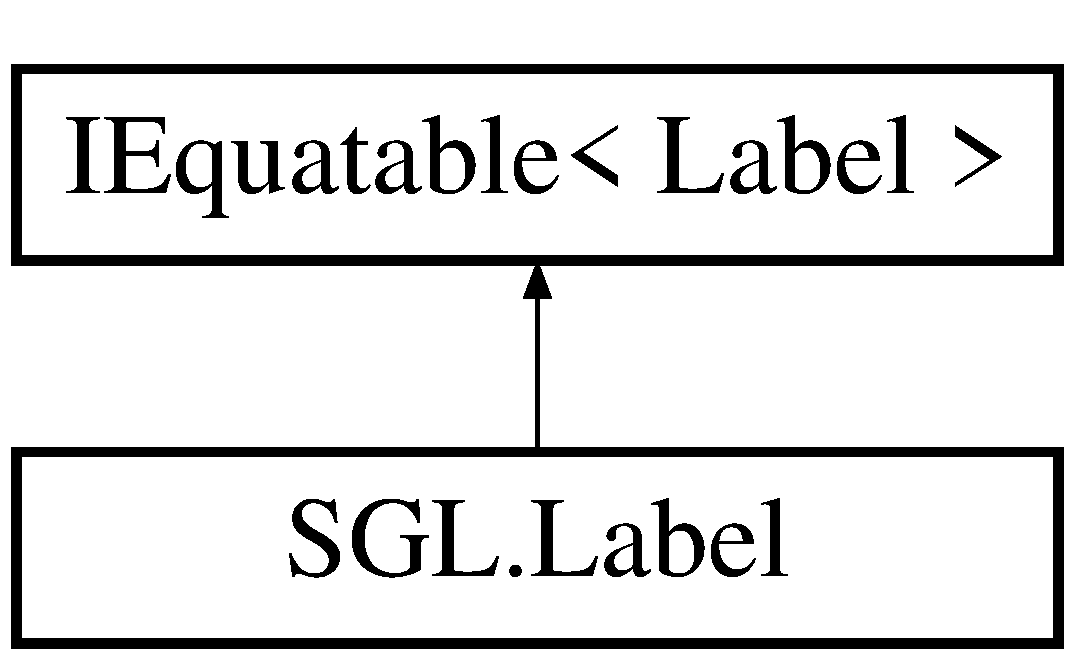
\includegraphics[height=2.000000cm]{class_s_g_l_1_1_label}
\end{center}
\end{figure}
\subsection*{Public Member Functions}
\begin{DoxyCompactItemize}
\item 
\mbox{\hyperlink{class_s_g_l_1_1_label_a1be3c869e06d8fc2da560a4fec1be8fd}{Label}} (\mbox{\hyperlink{struct_s_g_l_1_1_point}{Point}} position, string text, \mbox{\hyperlink{namespace_s_g_l_aa8de446c655c151ef21cfe27b24da87c}{Alignment}} alignment=Alignment.\+Top)
\begin{DoxyCompactList}\small\item\em Creates a label at the given position and with the given message and alignment. \end{DoxyCompactList}\item 
\mbox{\hyperlink{class_s_g_l_1_1_label_a11a9b6b3f98a52007ae874d22dc2f348}{Label}} (double x, double y, string text, \mbox{\hyperlink{namespace_s_g_l_aa8de446c655c151ef21cfe27b24da87c}{Alignment}} alignment=Alignment.\+Top)
\begin{DoxyCompactList}\small\item\em Creates a label at the given position and with the given message and alignment. \end{DoxyCompactList}\item 
\mbox{\Hypertarget{class_s_g_l_1_1_label_a68959b0181bc08450c2a5ba1a30df705}\label{class_s_g_l_1_1_label_a68959b0181bc08450c2a5ba1a30df705}} 
bool {\bfseries Equals} (\mbox{\hyperlink{class_s_g_l_1_1_label}{Label}} other)
\item 
\mbox{\Hypertarget{class_s_g_l_1_1_label_ab1f388c98f9e912195411337f7287c3c}\label{class_s_g_l_1_1_label_ab1f388c98f9e912195411337f7287c3c}} 
override bool {\bfseries Equals} (object obj)
\item 
\mbox{\Hypertarget{class_s_g_l_1_1_label_a256edbbb21ad2232fc73e2f7368b2b1d}\label{class_s_g_l_1_1_label_a256edbbb21ad2232fc73e2f7368b2b1d}} 
override int {\bfseries Get\+Hash\+Code} ()
\end{DoxyCompactItemize}
\subsection*{Static Public Member Functions}
\begin{DoxyCompactItemize}
\item 
\mbox{\Hypertarget{class_s_g_l_1_1_label_acfdcba6284f755436274b8b02497731e}\label{class_s_g_l_1_1_label_acfdcba6284f755436274b8b02497731e}} 
static bool {\bfseries operator==} (\mbox{\hyperlink{class_s_g_l_1_1_label}{Label}} a, \mbox{\hyperlink{class_s_g_l_1_1_label}{Label}} b)
\item 
\mbox{\Hypertarget{class_s_g_l_1_1_label_a33d5c6719db459ad98648c6a57bef735}\label{class_s_g_l_1_1_label_a33d5c6719db459ad98648c6a57bef735}} 
static bool {\bfseries operator!=} (\mbox{\hyperlink{class_s_g_l_1_1_label}{Label}} a, \mbox{\hyperlink{class_s_g_l_1_1_label}{Label}} b)
\end{DoxyCompactItemize}
\subsection*{Properties}
\begin{DoxyCompactItemize}
\item 
double \mbox{\hyperlink{class_s_g_l_1_1_label_adfba11f4ead1d6dd29785a7530acfca0}{X}}\hspace{0.3cm}{\ttfamily  \mbox{[}get, set\mbox{]}}
\begin{DoxyCompactList}\small\item\em The X-\/coordinate of the label. \end{DoxyCompactList}\item 
double \mbox{\hyperlink{class_s_g_l_1_1_label_a7c8067fe0098721a4a9cb6bd187e005d}{Y}}\hspace{0.3cm}{\ttfamily  \mbox{[}get, set\mbox{]}}
\begin{DoxyCompactList}\small\item\em The Y-\/coordinate of the label. \end{DoxyCompactList}\item 
\mbox{\hyperlink{struct_s_g_l_1_1_point}{Point}} \mbox{\hyperlink{class_s_g_l_1_1_label_a31dbcad567e6ef89d49f02eb55312308}{Position}}\hspace{0.3cm}{\ttfamily  \mbox{[}get, set\mbox{]}}
\begin{DoxyCompactList}\small\item\em The position of the label. \end{DoxyCompactList}\item 
string \mbox{\hyperlink{class_s_g_l_1_1_label_abc39b1a43ac82e057d716f3d2bc6056a}{Text}}\hspace{0.3cm}{\ttfamily  \mbox{[}get, set\mbox{]}}
\begin{DoxyCompactList}\small\item\em The text content of the label. \end{DoxyCompactList}\item 
\mbox{\hyperlink{namespace_s_g_l_aa8de446c655c151ef21cfe27b24da87c}{Alignment}} \mbox{\hyperlink{class_s_g_l_1_1_label_a00910f48f4a61d787308b77341ba9bcc}{Alignment}}\hspace{0.3cm}{\ttfamily  \mbox{[}get, set\mbox{]}}
\begin{DoxyCompactList}\small\item\em The alignment of the label relative to the point. \end{DoxyCompactList}\end{DoxyCompactItemize}


\subsection{Detailed Description}
Represent some text on the graph, defined by an origin point and a text message. 



\subsection{Constructor \& Destructor Documentation}
\mbox{\Hypertarget{class_s_g_l_1_1_label_a1be3c869e06d8fc2da560a4fec1be8fd}\label{class_s_g_l_1_1_label_a1be3c869e06d8fc2da560a4fec1be8fd}} 
\index{S\+G\+L\+::\+Label@{S\+G\+L\+::\+Label}!Label@{Label}}
\index{Label@{Label}!S\+G\+L\+::\+Label@{S\+G\+L\+::\+Label}}
\subsubsection{\texorpdfstring{Label()}{Label()}\hspace{0.1cm}{\footnotesize\ttfamily [1/2]}}
{\footnotesize\ttfamily S\+G\+L.\+Label.\+Label (\begin{DoxyParamCaption}\item[{\mbox{\hyperlink{struct_s_g_l_1_1_point}{Point}}}]{position,  }\item[{string}]{text,  }\item[{\mbox{\hyperlink{namespace_s_g_l_aa8de446c655c151ef21cfe27b24da87c}{Alignment}}}]{alignment = {\ttfamily Alignment.Top} }\end{DoxyParamCaption})\hspace{0.3cm}{\ttfamily [inline]}}



Creates a label at the given position and with the given message and alignment. 

\mbox{\Hypertarget{class_s_g_l_1_1_label_a11a9b6b3f98a52007ae874d22dc2f348}\label{class_s_g_l_1_1_label_a11a9b6b3f98a52007ae874d22dc2f348}} 
\index{S\+G\+L\+::\+Label@{S\+G\+L\+::\+Label}!Label@{Label}}
\index{Label@{Label}!S\+G\+L\+::\+Label@{S\+G\+L\+::\+Label}}
\subsubsection{\texorpdfstring{Label()}{Label()}\hspace{0.1cm}{\footnotesize\ttfamily [2/2]}}
{\footnotesize\ttfamily S\+G\+L.\+Label.\+Label (\begin{DoxyParamCaption}\item[{double}]{x,  }\item[{double}]{y,  }\item[{string}]{text,  }\item[{\mbox{\hyperlink{namespace_s_g_l_aa8de446c655c151ef21cfe27b24da87c}{Alignment}}}]{alignment = {\ttfamily Alignment.Top} }\end{DoxyParamCaption})\hspace{0.3cm}{\ttfamily [inline]}}



Creates a label at the given position and with the given message and alignment. 



\subsection{Property Documentation}
\mbox{\Hypertarget{class_s_g_l_1_1_label_a00910f48f4a61d787308b77341ba9bcc}\label{class_s_g_l_1_1_label_a00910f48f4a61d787308b77341ba9bcc}} 
\index{S\+G\+L\+::\+Label@{S\+G\+L\+::\+Label}!Alignment@{Alignment}}
\index{Alignment@{Alignment}!S\+G\+L\+::\+Label@{S\+G\+L\+::\+Label}}
\subsubsection{\texorpdfstring{Alignment}{Alignment}}
{\footnotesize\ttfamily \mbox{\hyperlink{namespace_s_g_l_aa8de446c655c151ef21cfe27b24da87c}{Alignment}} S\+G\+L.\+Label.\+Alignment\hspace{0.3cm}{\ttfamily [get]}, {\ttfamily [set]}}



The alignment of the label relative to the point. 

\mbox{\Hypertarget{class_s_g_l_1_1_label_a31dbcad567e6ef89d49f02eb55312308}\label{class_s_g_l_1_1_label_a31dbcad567e6ef89d49f02eb55312308}} 
\index{S\+G\+L\+::\+Label@{S\+G\+L\+::\+Label}!Position@{Position}}
\index{Position@{Position}!S\+G\+L\+::\+Label@{S\+G\+L\+::\+Label}}
\subsubsection{\texorpdfstring{Position}{Position}}
{\footnotesize\ttfamily \mbox{\hyperlink{struct_s_g_l_1_1_point}{Point}} S\+G\+L.\+Label.\+Position\hspace{0.3cm}{\ttfamily [get]}, {\ttfamily [set]}}



The position of the label. 

\mbox{\Hypertarget{class_s_g_l_1_1_label_abc39b1a43ac82e057d716f3d2bc6056a}\label{class_s_g_l_1_1_label_abc39b1a43ac82e057d716f3d2bc6056a}} 
\index{S\+G\+L\+::\+Label@{S\+G\+L\+::\+Label}!Text@{Text}}
\index{Text@{Text}!S\+G\+L\+::\+Label@{S\+G\+L\+::\+Label}}
\subsubsection{\texorpdfstring{Text}{Text}}
{\footnotesize\ttfamily string S\+G\+L.\+Label.\+Text\hspace{0.3cm}{\ttfamily [get]}, {\ttfamily [set]}}



The text content of the label. 

\mbox{\Hypertarget{class_s_g_l_1_1_label_adfba11f4ead1d6dd29785a7530acfca0}\label{class_s_g_l_1_1_label_adfba11f4ead1d6dd29785a7530acfca0}} 
\index{S\+G\+L\+::\+Label@{S\+G\+L\+::\+Label}!X@{X}}
\index{X@{X}!S\+G\+L\+::\+Label@{S\+G\+L\+::\+Label}}
\subsubsection{\texorpdfstring{X}{X}}
{\footnotesize\ttfamily double S\+G\+L.\+Label.\+X\hspace{0.3cm}{\ttfamily [get]}, {\ttfamily [set]}}



The X-\/coordinate of the label. 

\mbox{\Hypertarget{class_s_g_l_1_1_label_a7c8067fe0098721a4a9cb6bd187e005d}\label{class_s_g_l_1_1_label_a7c8067fe0098721a4a9cb6bd187e005d}} 
\index{S\+G\+L\+::\+Label@{S\+G\+L\+::\+Label}!Y@{Y}}
\index{Y@{Y}!S\+G\+L\+::\+Label@{S\+G\+L\+::\+Label}}
\subsubsection{\texorpdfstring{Y}{Y}}
{\footnotesize\ttfamily double S\+G\+L.\+Label.\+Y\hspace{0.3cm}{\ttfamily [get]}, {\ttfamily [set]}}



The Y-\/coordinate of the label. 



The documentation for this class was generated from the following file\+:\begin{DoxyCompactItemize}
\item 
Label.\+cs\end{DoxyCompactItemize}

\hypertarget{class_s_g_l_1_1_line}{}\section{S\+G\+L.\+Line Class Reference}
\label{class_s_g_l_1_1_line}\index{S\+G\+L.\+Line@{S\+G\+L.\+Line}}


Represent a line defined by two points.  


Inheritance diagram for S\+G\+L.\+Line\+:\begin{figure}[H]
\begin{center}
\leavevmode
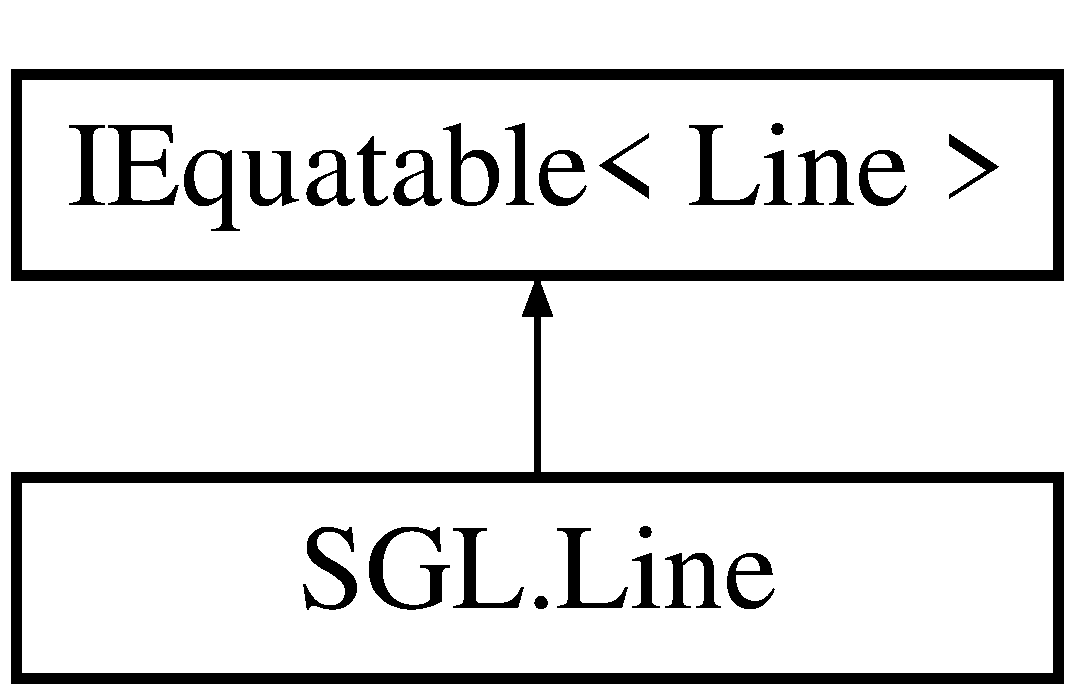
\includegraphics[height=2.000000cm]{class_s_g_l_1_1_line}
\end{center}
\end{figure}
\subsection*{Public Member Functions}
\begin{DoxyCompactItemize}
\item 
\mbox{\hyperlink{class_s_g_l_1_1_line_a8223479d92d17240ca099e57a3db2fb8}{Line}} (double x1, double y1, double x2, double y2)
\begin{DoxyCompactList}\small\item\em Creates a line between the two points. \end{DoxyCompactList}\item 
\mbox{\hyperlink{class_s_g_l_1_1_line_aa8638f980f735da597505f73105c8b44}{Line}} (\mbox{\hyperlink{struct_s_g_l_1_1_point}{Point}} a, \mbox{\hyperlink{struct_s_g_l_1_1_point}{Point}} b)
\begin{DoxyCompactList}\small\item\em Creates a line between the two points. \end{DoxyCompactList}\item 
\mbox{\Hypertarget{class_s_g_l_1_1_line_a843197ff24817c39a8640ef6a0fce6a6}\label{class_s_g_l_1_1_line_a843197ff24817c39a8640ef6a0fce6a6}} 
bool {\bfseries Equals} (\mbox{\hyperlink{class_s_g_l_1_1_line}{Line}} other)
\item 
\mbox{\Hypertarget{class_s_g_l_1_1_line_ac22009bbb59798ccdc5d456e8f460687}\label{class_s_g_l_1_1_line_ac22009bbb59798ccdc5d456e8f460687}} 
override bool {\bfseries Equals} (object obj)
\item 
\mbox{\Hypertarget{class_s_g_l_1_1_line_a0e1a9dfda6f68cc061f55d64364cde9c}\label{class_s_g_l_1_1_line_a0e1a9dfda6f68cc061f55d64364cde9c}} 
override int {\bfseries Get\+Hash\+Code} ()
\item 
\mbox{\Hypertarget{class_s_g_l_1_1_line_a10d26aa2ac7871020125a44032600455}\label{class_s_g_l_1_1_line_a10d26aa2ac7871020125a44032600455}} 
override string {\bfseries To\+String} ()
\end{DoxyCompactItemize}
\subsection*{Static Public Member Functions}
\begin{DoxyCompactItemize}
\item 
\mbox{\Hypertarget{class_s_g_l_1_1_line_a96549db302566a0e3e9d893c520edcb4}\label{class_s_g_l_1_1_line_a96549db302566a0e3e9d893c520edcb4}} 
static bool {\bfseries operator==} (\mbox{\hyperlink{class_s_g_l_1_1_line}{Line}} a, \mbox{\hyperlink{class_s_g_l_1_1_line}{Line}} b)
\item 
\mbox{\Hypertarget{class_s_g_l_1_1_line_a098603498d14698cac23a2d1daea73f8}\label{class_s_g_l_1_1_line_a098603498d14698cac23a2d1daea73f8}} 
static bool {\bfseries operator!=} (\mbox{\hyperlink{class_s_g_l_1_1_line}{Line}} a, \mbox{\hyperlink{class_s_g_l_1_1_line}{Line}} b)
\end{DoxyCompactItemize}
\subsection*{Public Attributes}
\begin{DoxyCompactItemize}
\item 
double \mbox{\hyperlink{class_s_g_l_1_1_line_a58ee417f43a6acd3b7c4f00c190c26fa}{Length}} =$>$ \mbox{\hyperlink{struct_s_g_l_1_1_point_a88dc45979fe8192615705469fc12f18b}{Point.\+Distance}}(\mbox{\hyperlink{class_s_g_l_1_1_line_a4485492024fc96d2db3aa34d699f974e}{X1}}, \mbox{\hyperlink{class_s_g_l_1_1_line_a1875f7240fd5be5323aaef118c9308c0}{Y1}}, \mbox{\hyperlink{class_s_g_l_1_1_line_ab6dcb09fcf8983e99c5230d4321bbfc8}{X2}}, \mbox{\hyperlink{class_s_g_l_1_1_line_af3571b932c09f78f70e288770e266341}{Y2}})
\begin{DoxyCompactList}\small\item\em Calculates the distance between the two ends of the line. \end{DoxyCompactList}\end{DoxyCompactItemize}
\subsection*{Properties}
\begin{DoxyCompactItemize}
\item 
\mbox{\hyperlink{struct_s_g_l_1_1_point}{Point}} \mbox{\hyperlink{class_s_g_l_1_1_line_ad062108c742ed94352ffbd24153e7125}{Start}}\hspace{0.3cm}{\ttfamily  \mbox{[}get, set\mbox{]}}
\begin{DoxyCompactList}\small\item\em The starting point of the line. \end{DoxyCompactList}\item 
\mbox{\hyperlink{struct_s_g_l_1_1_point}{Point}} \mbox{\hyperlink{class_s_g_l_1_1_line_a6b6a840b2b8ce27ed017946da182a10e}{End}}\hspace{0.3cm}{\ttfamily  \mbox{[}get, set\mbox{]}}
\begin{DoxyCompactList}\small\item\em The ending point of the line. \end{DoxyCompactList}\item 
double \mbox{\hyperlink{class_s_g_l_1_1_line_a4485492024fc96d2db3aa34d699f974e}{X1}}\hspace{0.3cm}{\ttfamily  \mbox{[}get, set\mbox{]}}
\begin{DoxyCompactList}\small\item\em The X coordinate of the starting point. \end{DoxyCompactList}\item 
double \mbox{\hyperlink{class_s_g_l_1_1_line_ab6dcb09fcf8983e99c5230d4321bbfc8}{X2}}\hspace{0.3cm}{\ttfamily  \mbox{[}get, set\mbox{]}}
\begin{DoxyCompactList}\small\item\em The X coordinate of the ending point. \end{DoxyCompactList}\item 
double \mbox{\hyperlink{class_s_g_l_1_1_line_a1875f7240fd5be5323aaef118c9308c0}{Y1}}\hspace{0.3cm}{\ttfamily  \mbox{[}get, set\mbox{]}}
\begin{DoxyCompactList}\small\item\em The Y coordinate of the starting point. \end{DoxyCompactList}\item 
double \mbox{\hyperlink{class_s_g_l_1_1_line_af3571b932c09f78f70e288770e266341}{Y2}}\hspace{0.3cm}{\ttfamily  \mbox{[}get, set\mbox{]}}
\begin{DoxyCompactList}\small\item\em The Y coordinate of the ending point. \end{DoxyCompactList}\end{DoxyCompactItemize}


\subsection{Detailed Description}
Represent a line defined by two points. 



\subsection{Constructor \& Destructor Documentation}
\mbox{\Hypertarget{class_s_g_l_1_1_line_a8223479d92d17240ca099e57a3db2fb8}\label{class_s_g_l_1_1_line_a8223479d92d17240ca099e57a3db2fb8}} 
\index{S\+G\+L\+::\+Line@{S\+G\+L\+::\+Line}!Line@{Line}}
\index{Line@{Line}!S\+G\+L\+::\+Line@{S\+G\+L\+::\+Line}}
\subsubsection{\texorpdfstring{Line()}{Line()}\hspace{0.1cm}{\footnotesize\ttfamily [1/2]}}
{\footnotesize\ttfamily S\+G\+L.\+Line.\+Line (\begin{DoxyParamCaption}\item[{double}]{x1,  }\item[{double}]{y1,  }\item[{double}]{x2,  }\item[{double}]{y2 }\end{DoxyParamCaption})\hspace{0.3cm}{\ttfamily [inline]}}



Creates a line between the two points. 

\mbox{\Hypertarget{class_s_g_l_1_1_line_aa8638f980f735da597505f73105c8b44}\label{class_s_g_l_1_1_line_aa8638f980f735da597505f73105c8b44}} 
\index{S\+G\+L\+::\+Line@{S\+G\+L\+::\+Line}!Line@{Line}}
\index{Line@{Line}!S\+G\+L\+::\+Line@{S\+G\+L\+::\+Line}}
\subsubsection{\texorpdfstring{Line()}{Line()}\hspace{0.1cm}{\footnotesize\ttfamily [2/2]}}
{\footnotesize\ttfamily S\+G\+L.\+Line.\+Line (\begin{DoxyParamCaption}\item[{\mbox{\hyperlink{struct_s_g_l_1_1_point}{Point}}}]{a,  }\item[{\mbox{\hyperlink{struct_s_g_l_1_1_point}{Point}}}]{b }\end{DoxyParamCaption})\hspace{0.3cm}{\ttfamily [inline]}}



Creates a line between the two points. 



\subsection{Member Data Documentation}
\mbox{\Hypertarget{class_s_g_l_1_1_line_a58ee417f43a6acd3b7c4f00c190c26fa}\label{class_s_g_l_1_1_line_a58ee417f43a6acd3b7c4f00c190c26fa}} 
\index{S\+G\+L\+::\+Line@{S\+G\+L\+::\+Line}!Length@{Length}}
\index{Length@{Length}!S\+G\+L\+::\+Line@{S\+G\+L\+::\+Line}}
\subsubsection{\texorpdfstring{Length}{Length}}
{\footnotesize\ttfamily double S\+G\+L.\+Line.\+Length =$>$ \mbox{\hyperlink{struct_s_g_l_1_1_point_a88dc45979fe8192615705469fc12f18b}{Point.\+Distance}}(\mbox{\hyperlink{class_s_g_l_1_1_line_a4485492024fc96d2db3aa34d699f974e}{X1}}, \mbox{\hyperlink{class_s_g_l_1_1_line_a1875f7240fd5be5323aaef118c9308c0}{Y1}}, \mbox{\hyperlink{class_s_g_l_1_1_line_ab6dcb09fcf8983e99c5230d4321bbfc8}{X2}}, \mbox{\hyperlink{class_s_g_l_1_1_line_af3571b932c09f78f70e288770e266341}{Y2}})}



Calculates the distance between the two ends of the line. 



\subsection{Property Documentation}
\mbox{\Hypertarget{class_s_g_l_1_1_line_a6b6a840b2b8ce27ed017946da182a10e}\label{class_s_g_l_1_1_line_a6b6a840b2b8ce27ed017946da182a10e}} 
\index{S\+G\+L\+::\+Line@{S\+G\+L\+::\+Line}!End@{End}}
\index{End@{End}!S\+G\+L\+::\+Line@{S\+G\+L\+::\+Line}}
\subsubsection{\texorpdfstring{End}{End}}
{\footnotesize\ttfamily \mbox{\hyperlink{struct_s_g_l_1_1_point}{Point}} S\+G\+L.\+Line.\+End\hspace{0.3cm}{\ttfamily [get]}, {\ttfamily [set]}}



The ending point of the line. 

\mbox{\Hypertarget{class_s_g_l_1_1_line_ad062108c742ed94352ffbd24153e7125}\label{class_s_g_l_1_1_line_ad062108c742ed94352ffbd24153e7125}} 
\index{S\+G\+L\+::\+Line@{S\+G\+L\+::\+Line}!Start@{Start}}
\index{Start@{Start}!S\+G\+L\+::\+Line@{S\+G\+L\+::\+Line}}
\subsubsection{\texorpdfstring{Start}{Start}}
{\footnotesize\ttfamily \mbox{\hyperlink{struct_s_g_l_1_1_point}{Point}} S\+G\+L.\+Line.\+Start\hspace{0.3cm}{\ttfamily [get]}, {\ttfamily [set]}}



The starting point of the line. 

\mbox{\Hypertarget{class_s_g_l_1_1_line_a4485492024fc96d2db3aa34d699f974e}\label{class_s_g_l_1_1_line_a4485492024fc96d2db3aa34d699f974e}} 
\index{S\+G\+L\+::\+Line@{S\+G\+L\+::\+Line}!X1@{X1}}
\index{X1@{X1}!S\+G\+L\+::\+Line@{S\+G\+L\+::\+Line}}
\subsubsection{\texorpdfstring{X1}{X1}}
{\footnotesize\ttfamily double S\+G\+L.\+Line.\+X1\hspace{0.3cm}{\ttfamily [get]}, {\ttfamily [set]}}



The X coordinate of the starting point. 

\mbox{\Hypertarget{class_s_g_l_1_1_line_ab6dcb09fcf8983e99c5230d4321bbfc8}\label{class_s_g_l_1_1_line_ab6dcb09fcf8983e99c5230d4321bbfc8}} 
\index{S\+G\+L\+::\+Line@{S\+G\+L\+::\+Line}!X2@{X2}}
\index{X2@{X2}!S\+G\+L\+::\+Line@{S\+G\+L\+::\+Line}}
\subsubsection{\texorpdfstring{X2}{X2}}
{\footnotesize\ttfamily double S\+G\+L.\+Line.\+X2\hspace{0.3cm}{\ttfamily [get]}, {\ttfamily [set]}}



The X coordinate of the ending point. 

\mbox{\Hypertarget{class_s_g_l_1_1_line_a1875f7240fd5be5323aaef118c9308c0}\label{class_s_g_l_1_1_line_a1875f7240fd5be5323aaef118c9308c0}} 
\index{S\+G\+L\+::\+Line@{S\+G\+L\+::\+Line}!Y1@{Y1}}
\index{Y1@{Y1}!S\+G\+L\+::\+Line@{S\+G\+L\+::\+Line}}
\subsubsection{\texorpdfstring{Y1}{Y1}}
{\footnotesize\ttfamily double S\+G\+L.\+Line.\+Y1\hspace{0.3cm}{\ttfamily [get]}, {\ttfamily [set]}}



The Y coordinate of the starting point. 

\mbox{\Hypertarget{class_s_g_l_1_1_line_af3571b932c09f78f70e288770e266341}\label{class_s_g_l_1_1_line_af3571b932c09f78f70e288770e266341}} 
\index{S\+G\+L\+::\+Line@{S\+G\+L\+::\+Line}!Y2@{Y2}}
\index{Y2@{Y2}!S\+G\+L\+::\+Line@{S\+G\+L\+::\+Line}}
\subsubsection{\texorpdfstring{Y2}{Y2}}
{\footnotesize\ttfamily double S\+G\+L.\+Line.\+Y2\hspace{0.3cm}{\ttfamily [get]}, {\ttfamily [set]}}



The Y coordinate of the ending point. 



The documentation for this class was generated from the following file\+:\begin{DoxyCompactItemize}
\item 
Line.\+cs\end{DoxyCompactItemize}

\hypertarget{struct_s_g_l_1_1_point}{}\section{S\+G\+L.\+Point Struct Reference}
\label{struct_s_g_l_1_1_point}\index{S\+G\+L.\+Point@{S\+G\+L.\+Point}}


Represent a point defined by two coordinates (X and Y).  


Inheritance diagram for S\+G\+L.\+Point\+:\begin{figure}[H]
\begin{center}
\leavevmode
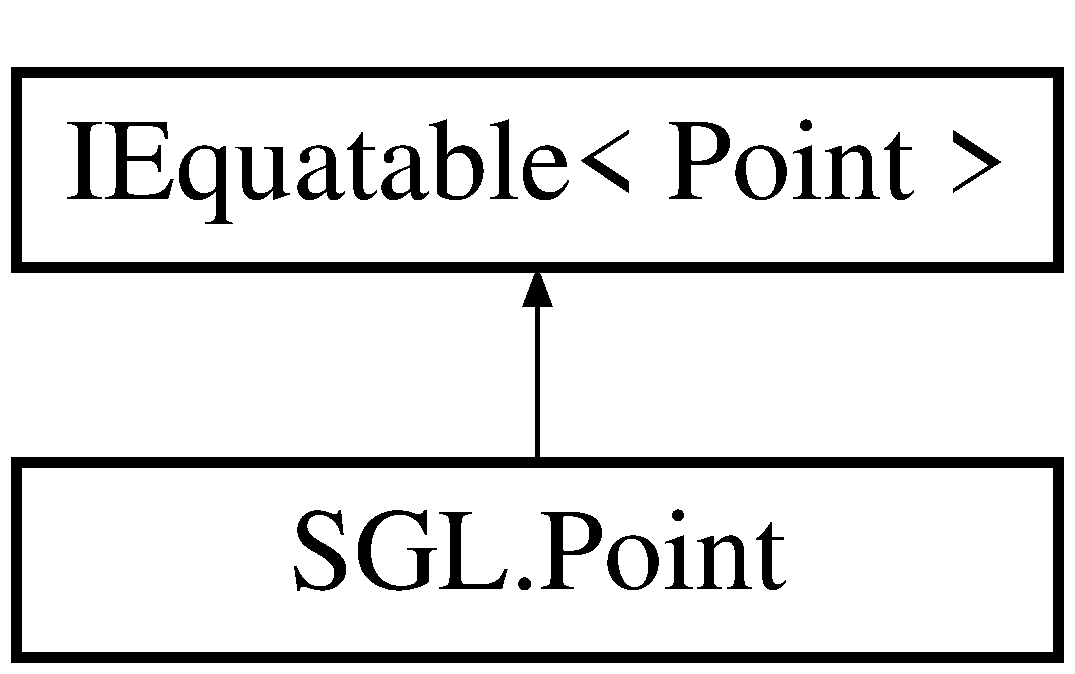
\includegraphics[height=2.000000cm]{struct_s_g_l_1_1_point}
\end{center}
\end{figure}
\subsection*{Public Member Functions}
\begin{DoxyCompactItemize}
\item 
\mbox{\hyperlink{struct_s_g_l_1_1_point_a56c9ba13f3b84483a108ae16fc635cac}{Point}} (double x, double y)
\begin{DoxyCompactList}\small\item\em Creates a point with the given coorinates. \end{DoxyCompactList}\item 
double \mbox{\hyperlink{struct_s_g_l_1_1_point_aa44e48a67f96810b5483955a80426442}{Distance}} (\mbox{\hyperlink{struct_s_g_l_1_1_point}{Point}} other)
\begin{DoxyCompactList}\small\item\em Calculates the distance from one point to another. \end{DoxyCompactList}\item 
\mbox{\hyperlink{struct_s_g_l_1_1_point}{Point}} \mbox{\hyperlink{struct_s_g_l_1_1_point_a4680568d8a9b123e6ffaf27ec22030ff}{Lerp}} (\mbox{\hyperlink{struct_s_g_l_1_1_point}{Point}} value2, double amount)
\begin{DoxyCompactList}\small\item\em Linearly interpolates between the two points by the specified amount. Returns {\itshape value1}  for 0, {\itshape value2}  for 1. \end{DoxyCompactList}\item 
\mbox{\Hypertarget{struct_s_g_l_1_1_point_a87c11e4e715447147db175bf1542aa9b}\label{struct_s_g_l_1_1_point_a87c11e4e715447147db175bf1542aa9b}} 
bool {\bfseries Equals} (\mbox{\hyperlink{struct_s_g_l_1_1_point}{Point}} other)
\item 
\mbox{\Hypertarget{struct_s_g_l_1_1_point_acc67f296d3dfae3982f618f9deeaafe7}\label{struct_s_g_l_1_1_point_acc67f296d3dfae3982f618f9deeaafe7}} 
override bool {\bfseries Equals} (object obj)
\item 
\mbox{\Hypertarget{struct_s_g_l_1_1_point_a5d9b1d1e671a738b93f8b8d81f755fc6}\label{struct_s_g_l_1_1_point_a5d9b1d1e671a738b93f8b8d81f755fc6}} 
override int {\bfseries Get\+Hash\+Code} ()
\item 
\mbox{\Hypertarget{struct_s_g_l_1_1_point_aefc624c50fcac9e87f657e43c39213d6}\label{struct_s_g_l_1_1_point_aefc624c50fcac9e87f657e43c39213d6}} 
override string {\bfseries To\+String} ()
\end{DoxyCompactItemize}
\subsection*{Static Public Member Functions}
\begin{DoxyCompactItemize}
\item 
\mbox{\Hypertarget{struct_s_g_l_1_1_point_a1f03b9dc317808ffceac4a8b65443d10}\label{struct_s_g_l_1_1_point_a1f03b9dc317808ffceac4a8b65443d10}} 
static \mbox{\hyperlink{struct_s_g_l_1_1_point}{Point}} {\bfseries operator-\/} (\mbox{\hyperlink{struct_s_g_l_1_1_point}{Point}} p)
\item 
\mbox{\Hypertarget{struct_s_g_l_1_1_point_a27314b0efd592b31cef2f58b3d17e74e}\label{struct_s_g_l_1_1_point_a27314b0efd592b31cef2f58b3d17e74e}} 
static \mbox{\hyperlink{struct_s_g_l_1_1_point}{Point}} {\bfseries operator+} (\mbox{\hyperlink{struct_s_g_l_1_1_point}{Point}} a, \mbox{\hyperlink{struct_s_g_l_1_1_point}{Point}} b)
\item 
\mbox{\Hypertarget{struct_s_g_l_1_1_point_a3a06ac359ac9d1af2aefef9874ef6d3b}\label{struct_s_g_l_1_1_point_a3a06ac359ac9d1af2aefef9874ef6d3b}} 
static \mbox{\hyperlink{struct_s_g_l_1_1_point}{Point}} {\bfseries operator-\/} (\mbox{\hyperlink{struct_s_g_l_1_1_point}{Point}} a, \mbox{\hyperlink{struct_s_g_l_1_1_point}{Point}} b)
\item 
\mbox{\Hypertarget{struct_s_g_l_1_1_point_ad326976c9346f26566388898f9049ac6}\label{struct_s_g_l_1_1_point_ad326976c9346f26566388898f9049ac6}} 
static \mbox{\hyperlink{struct_s_g_l_1_1_point}{Point}} {\bfseries operator$\ast$} (\mbox{\hyperlink{struct_s_g_l_1_1_point}{Point}} p, double value)
\item 
\mbox{\Hypertarget{struct_s_g_l_1_1_point_a6d529ac9b58ac7fef196be302b8d5ac0}\label{struct_s_g_l_1_1_point_a6d529ac9b58ac7fef196be302b8d5ac0}} 
static \mbox{\hyperlink{struct_s_g_l_1_1_point}{Point}} {\bfseries operator/} (\mbox{\hyperlink{struct_s_g_l_1_1_point}{Point}} p, double value)
\item 
static double \mbox{\hyperlink{struct_s_g_l_1_1_point_a88dc45979fe8192615705469fc12f18b}{Distance}} (double x1, double y1, double x2, double y2)
\begin{DoxyCompactList}\small\item\em Calculates the distance from one point to another. \end{DoxyCompactList}\item 
\mbox{\Hypertarget{struct_s_g_l_1_1_point_a1df0fcbce5751738c6e2ce49bb5e3348}\label{struct_s_g_l_1_1_point_a1df0fcbce5751738c6e2ce49bb5e3348}} 
static bool {\bfseries operator==} (\mbox{\hyperlink{struct_s_g_l_1_1_point}{Point}} a, \mbox{\hyperlink{struct_s_g_l_1_1_point}{Point}} b)
\item 
\mbox{\Hypertarget{struct_s_g_l_1_1_point_a3dd8c199fe7f90ba9ae0b1db6ea49a48}\label{struct_s_g_l_1_1_point_a3dd8c199fe7f90ba9ae0b1db6ea49a48}} 
static bool {\bfseries operator!=} (\mbox{\hyperlink{struct_s_g_l_1_1_point}{Point}} a, \mbox{\hyperlink{struct_s_g_l_1_1_point}{Point}} b)
\end{DoxyCompactItemize}
\subsection*{Static Public Attributes}
\begin{DoxyCompactItemize}
\item 
static \mbox{\hyperlink{struct_s_g_l_1_1_point}{Point}} \mbox{\hyperlink{struct_s_g_l_1_1_point_a4dd7959c1b84f270da8c3b51c2bc0a11}{Origin}} =$>$ new \mbox{\hyperlink{struct_s_g_l_1_1_point}{Point}}(0, 0)
\begin{DoxyCompactList}\small\item\em The origin point (0, 0). \end{DoxyCompactList}\item 
static \mbox{\hyperlink{struct_s_g_l_1_1_point}{Point}} \mbox{\hyperlink{struct_s_g_l_1_1_point_a08d6f7dd7dfb57c6e1be9ce0e7843b9d}{Up}} =$>$ new \mbox{\hyperlink{struct_s_g_l_1_1_point}{Point}}(0, 1)
\begin{DoxyCompactList}\small\item\em The point (0, 1). \end{DoxyCompactList}\item 
static \mbox{\hyperlink{struct_s_g_l_1_1_point}{Point}} \mbox{\hyperlink{struct_s_g_l_1_1_point_a0bc08cef11531d4036aa895d2c33af1e}{Down}} =$>$ new \mbox{\hyperlink{struct_s_g_l_1_1_point}{Point}}(0, -\/1)
\begin{DoxyCompactList}\small\item\em The point (0, -\/1). \end{DoxyCompactList}\item 
static \mbox{\hyperlink{struct_s_g_l_1_1_point}{Point}} \mbox{\hyperlink{struct_s_g_l_1_1_point_a26624170987d06859725b637117fa211}{Left}} =$>$ new \mbox{\hyperlink{struct_s_g_l_1_1_point}{Point}}(-\/1, 0)
\begin{DoxyCompactList}\small\item\em The point (-\/1, 0). \end{DoxyCompactList}\item 
static \mbox{\hyperlink{struct_s_g_l_1_1_point}{Point}} \mbox{\hyperlink{struct_s_g_l_1_1_point_a320d6bfd5119b652d958b5f72e2f737c}{Right}} =$>$ new \mbox{\hyperlink{struct_s_g_l_1_1_point}{Point}}(1, 0)
\begin{DoxyCompactList}\small\item\em The point (0, 1). \end{DoxyCompactList}\end{DoxyCompactItemize}
\subsection*{Properties}
\begin{DoxyCompactItemize}
\item 
\mbox{\Hypertarget{struct_s_g_l_1_1_point_a762ce7cac4f0081373601711ff2cfde2}\label{struct_s_g_l_1_1_point_a762ce7cac4f0081373601711ff2cfde2}} 
double {\bfseries X}\hspace{0.3cm}{\ttfamily  \mbox{[}get, set\mbox{]}}
\item 
\mbox{\Hypertarget{struct_s_g_l_1_1_point_a53213a574ab4d3bbea18216a193b6a54}\label{struct_s_g_l_1_1_point_a53213a574ab4d3bbea18216a193b6a54}} 
double {\bfseries Y}\hspace{0.3cm}{\ttfamily  \mbox{[}get, set\mbox{]}}
\end{DoxyCompactItemize}


\subsection{Detailed Description}
Represent a point defined by two coordinates (X and Y). 



\subsection{Constructor \& Destructor Documentation}
\mbox{\Hypertarget{struct_s_g_l_1_1_point_a56c9ba13f3b84483a108ae16fc635cac}\label{struct_s_g_l_1_1_point_a56c9ba13f3b84483a108ae16fc635cac}} 
\index{S\+G\+L\+::\+Point@{S\+G\+L\+::\+Point}!Point@{Point}}
\index{Point@{Point}!S\+G\+L\+::\+Point@{S\+G\+L\+::\+Point}}
\subsubsection{\texorpdfstring{Point()}{Point()}}
{\footnotesize\ttfamily S\+G\+L.\+Point.\+Point (\begin{DoxyParamCaption}\item[{double}]{x,  }\item[{double}]{y }\end{DoxyParamCaption})\hspace{0.3cm}{\ttfamily [inline]}}



Creates a point with the given coorinates. 



\subsection{Member Function Documentation}
\mbox{\Hypertarget{struct_s_g_l_1_1_point_a88dc45979fe8192615705469fc12f18b}\label{struct_s_g_l_1_1_point_a88dc45979fe8192615705469fc12f18b}} 
\index{S\+G\+L\+::\+Point@{S\+G\+L\+::\+Point}!Distance@{Distance}}
\index{Distance@{Distance}!S\+G\+L\+::\+Point@{S\+G\+L\+::\+Point}}
\subsubsection{\texorpdfstring{Distance()}{Distance()}\hspace{0.1cm}{\footnotesize\ttfamily [1/2]}}
{\footnotesize\ttfamily static double S\+G\+L.\+Point.\+Distance (\begin{DoxyParamCaption}\item[{double}]{x1,  }\item[{double}]{y1,  }\item[{double}]{x2,  }\item[{double}]{y2 }\end{DoxyParamCaption})\hspace{0.3cm}{\ttfamily [inline]}, {\ttfamily [static]}}



Calculates the distance from one point to another. 

\mbox{\Hypertarget{struct_s_g_l_1_1_point_aa44e48a67f96810b5483955a80426442}\label{struct_s_g_l_1_1_point_aa44e48a67f96810b5483955a80426442}} 
\index{S\+G\+L\+::\+Point@{S\+G\+L\+::\+Point}!Distance@{Distance}}
\index{Distance@{Distance}!S\+G\+L\+::\+Point@{S\+G\+L\+::\+Point}}
\subsubsection{\texorpdfstring{Distance()}{Distance()}\hspace{0.1cm}{\footnotesize\ttfamily [2/2]}}
{\footnotesize\ttfamily double S\+G\+L.\+Point.\+Distance (\begin{DoxyParamCaption}\item[{\mbox{\hyperlink{struct_s_g_l_1_1_point}{Point}}}]{other }\end{DoxyParamCaption})\hspace{0.3cm}{\ttfamily [inline]}}



Calculates the distance from one point to another. 

\mbox{\Hypertarget{struct_s_g_l_1_1_point_a4680568d8a9b123e6ffaf27ec22030ff}\label{struct_s_g_l_1_1_point_a4680568d8a9b123e6ffaf27ec22030ff}} 
\index{S\+G\+L\+::\+Point@{S\+G\+L\+::\+Point}!Lerp@{Lerp}}
\index{Lerp@{Lerp}!S\+G\+L\+::\+Point@{S\+G\+L\+::\+Point}}
\subsubsection{\texorpdfstring{Lerp()}{Lerp()}}
{\footnotesize\ttfamily \mbox{\hyperlink{struct_s_g_l_1_1_point}{Point}} S\+G\+L.\+Point.\+Lerp (\begin{DoxyParamCaption}\item[{\mbox{\hyperlink{struct_s_g_l_1_1_point}{Point}}}]{value2,  }\item[{double}]{amount }\end{DoxyParamCaption})\hspace{0.3cm}{\ttfamily [inline]}}



Linearly interpolates between the two points by the specified amount. Returns {\itshape value1}  for 0, {\itshape value2}  for 1. 



\subsection{Member Data Documentation}
\mbox{\Hypertarget{struct_s_g_l_1_1_point_a0bc08cef11531d4036aa895d2c33af1e}\label{struct_s_g_l_1_1_point_a0bc08cef11531d4036aa895d2c33af1e}} 
\index{S\+G\+L\+::\+Point@{S\+G\+L\+::\+Point}!Down@{Down}}
\index{Down@{Down}!S\+G\+L\+::\+Point@{S\+G\+L\+::\+Point}}
\subsubsection{\texorpdfstring{Down}{Down}}
{\footnotesize\ttfamily \mbox{\hyperlink{struct_s_g_l_1_1_point}{Point}} S\+G\+L.\+Point.\+Down =$>$ new \mbox{\hyperlink{struct_s_g_l_1_1_point}{Point}}(0, -\/1)\hspace{0.3cm}{\ttfamily [static]}}



The point (0, -\/1). 

\mbox{\Hypertarget{struct_s_g_l_1_1_point_a26624170987d06859725b637117fa211}\label{struct_s_g_l_1_1_point_a26624170987d06859725b637117fa211}} 
\index{S\+G\+L\+::\+Point@{S\+G\+L\+::\+Point}!Left@{Left}}
\index{Left@{Left}!S\+G\+L\+::\+Point@{S\+G\+L\+::\+Point}}
\subsubsection{\texorpdfstring{Left}{Left}}
{\footnotesize\ttfamily \mbox{\hyperlink{struct_s_g_l_1_1_point}{Point}} S\+G\+L.\+Point.\+Left =$>$ new \mbox{\hyperlink{struct_s_g_l_1_1_point}{Point}}(-\/1, 0)\hspace{0.3cm}{\ttfamily [static]}}



The point (-\/1, 0). 

\mbox{\Hypertarget{struct_s_g_l_1_1_point_a4dd7959c1b84f270da8c3b51c2bc0a11}\label{struct_s_g_l_1_1_point_a4dd7959c1b84f270da8c3b51c2bc0a11}} 
\index{S\+G\+L\+::\+Point@{S\+G\+L\+::\+Point}!Origin@{Origin}}
\index{Origin@{Origin}!S\+G\+L\+::\+Point@{S\+G\+L\+::\+Point}}
\subsubsection{\texorpdfstring{Origin}{Origin}}
{\footnotesize\ttfamily \mbox{\hyperlink{struct_s_g_l_1_1_point}{Point}} S\+G\+L.\+Point.\+Origin =$>$ new \mbox{\hyperlink{struct_s_g_l_1_1_point}{Point}}(0, 0)\hspace{0.3cm}{\ttfamily [static]}}



The origin point (0, 0). 

\mbox{\Hypertarget{struct_s_g_l_1_1_point_a320d6bfd5119b652d958b5f72e2f737c}\label{struct_s_g_l_1_1_point_a320d6bfd5119b652d958b5f72e2f737c}} 
\index{S\+G\+L\+::\+Point@{S\+G\+L\+::\+Point}!Right@{Right}}
\index{Right@{Right}!S\+G\+L\+::\+Point@{S\+G\+L\+::\+Point}}
\subsubsection{\texorpdfstring{Right}{Right}}
{\footnotesize\ttfamily \mbox{\hyperlink{struct_s_g_l_1_1_point}{Point}} S\+G\+L.\+Point.\+Right =$>$ new \mbox{\hyperlink{struct_s_g_l_1_1_point}{Point}}(1, 0)\hspace{0.3cm}{\ttfamily [static]}}



The point (0, 1). 

\mbox{\Hypertarget{struct_s_g_l_1_1_point_a08d6f7dd7dfb57c6e1be9ce0e7843b9d}\label{struct_s_g_l_1_1_point_a08d6f7dd7dfb57c6e1be9ce0e7843b9d}} 
\index{S\+G\+L\+::\+Point@{S\+G\+L\+::\+Point}!Up@{Up}}
\index{Up@{Up}!S\+G\+L\+::\+Point@{S\+G\+L\+::\+Point}}
\subsubsection{\texorpdfstring{Up}{Up}}
{\footnotesize\ttfamily \mbox{\hyperlink{struct_s_g_l_1_1_point}{Point}} S\+G\+L.\+Point.\+Up =$>$ new \mbox{\hyperlink{struct_s_g_l_1_1_point}{Point}}(0, 1)\hspace{0.3cm}{\ttfamily [static]}}



The point (0, 1). 



The documentation for this struct was generated from the following file\+:\begin{DoxyCompactItemize}
\item 
Point.\+cs\end{DoxyCompactItemize}

\hypertarget{class_s_g_l_1_1_rectangle}{}\section{S\+G\+L.\+Rectangle Class Reference}
\label{class_s_g_l_1_1_rectangle}\index{S\+G\+L.\+Rectangle@{S\+G\+L.\+Rectangle}}


Represent a rectangle defined by its center and side dimensions.  


Inheritance diagram for S\+G\+L.\+Rectangle\+:\begin{figure}[H]
\begin{center}
\leavevmode
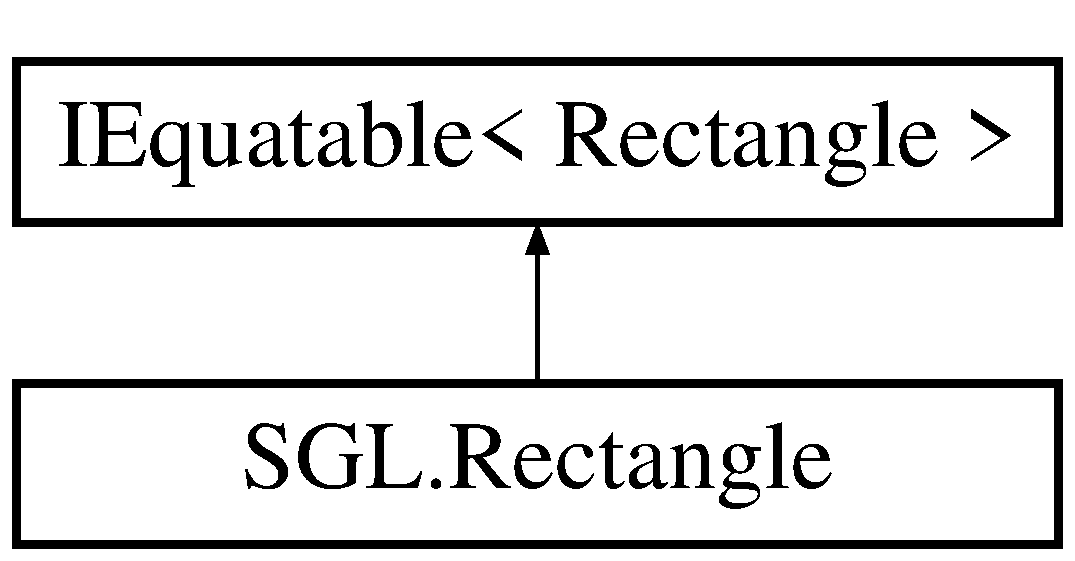
\includegraphics[height=2.000000cm]{class_s_g_l_1_1_rectangle}
\end{center}
\end{figure}
\subsection*{Public Member Functions}
\begin{DoxyCompactItemize}
\item 
\mbox{\Hypertarget{class_s_g_l_1_1_rectangle_a434c1422826c0ca43b7d4cd269f36c77}\label{class_s_g_l_1_1_rectangle_a434c1422826c0ca43b7d4cd269f36c77}} 
{\bfseries Rectangle} (double x, double y, double width, double height)
\item 
\mbox{\Hypertarget{class_s_g_l_1_1_rectangle_ab483c2330a3e5b46236e5b11d2a7bd90}\label{class_s_g_l_1_1_rectangle_ab483c2330a3e5b46236e5b11d2a7bd90}} 
{\bfseries Rectangle} (\mbox{\hyperlink{struct_s_g_l_1_1_point}{Point}} center, double width, double height)
\item 
\mbox{\Hypertarget{class_s_g_l_1_1_rectangle_a46cb3c0ffdcc2e5ba34fd567cafaff5c}\label{class_s_g_l_1_1_rectangle_a46cb3c0ffdcc2e5ba34fd567cafaff5c}} 
bool {\bfseries Contains} (\mbox{\hyperlink{struct_s_g_l_1_1_point}{Point}} p)
\item 
\mbox{\Hypertarget{class_s_g_l_1_1_rectangle_ade356368b8bc714fba5420b3996bd69f}\label{class_s_g_l_1_1_rectangle_ade356368b8bc714fba5420b3996bd69f}} 
bool {\bfseries Equals} (\mbox{\hyperlink{class_s_g_l_1_1_rectangle}{Rectangle}} other)
\item 
\mbox{\Hypertarget{class_s_g_l_1_1_rectangle_a4d8163b12df6d3bb94afcbd750e970d8}\label{class_s_g_l_1_1_rectangle_a4d8163b12df6d3bb94afcbd750e970d8}} 
override bool {\bfseries Equals} (object obj)
\item 
\mbox{\Hypertarget{class_s_g_l_1_1_rectangle_aa75086e37d8fbe1d62d147a017de4e37}\label{class_s_g_l_1_1_rectangle_aa75086e37d8fbe1d62d147a017de4e37}} 
override int {\bfseries Get\+Hash\+Code} ()
\item 
\mbox{\Hypertarget{class_s_g_l_1_1_rectangle_aa0e5c1a75a41412c7c7df8b037f667f9}\label{class_s_g_l_1_1_rectangle_aa0e5c1a75a41412c7c7df8b037f667f9}} 
override string {\bfseries To\+String} ()
\end{DoxyCompactItemize}
\subsection*{Static Public Member Functions}
\begin{DoxyCompactItemize}
\item 
\mbox{\Hypertarget{class_s_g_l_1_1_rectangle_ae3cb95607d2ca2ba4b963e1e8cb27455}\label{class_s_g_l_1_1_rectangle_ae3cb95607d2ca2ba4b963e1e8cb27455}} 
static bool {\bfseries operator==} (\mbox{\hyperlink{class_s_g_l_1_1_rectangle}{Rectangle}} a, \mbox{\hyperlink{class_s_g_l_1_1_rectangle}{Rectangle}} b)
\item 
\mbox{\Hypertarget{class_s_g_l_1_1_rectangle_a0c05f32a38285138e07df100f598ac5f}\label{class_s_g_l_1_1_rectangle_a0c05f32a38285138e07df100f598ac5f}} 
static bool {\bfseries operator!=} (\mbox{\hyperlink{class_s_g_l_1_1_rectangle}{Rectangle}} a, \mbox{\hyperlink{class_s_g_l_1_1_rectangle}{Rectangle}} b)
\end{DoxyCompactItemize}
\subsection*{Public Attributes}
\begin{DoxyCompactItemize}
\item 
double \mbox{\hyperlink{class_s_g_l_1_1_rectangle_ac84a60fb0f1f84cc3f36e488e5aafc29}{Area}} =$>$ \mbox{\hyperlink{class_s_g_l_1_1_rectangle_a717f64d0b1a88f2901ebb53bf5fdac72}{Width}} $\ast$ \mbox{\hyperlink{class_s_g_l_1_1_rectangle_ae241fbf3d3bc711d0046d10e1954baa2}{Height}}
\begin{DoxyCompactList}\small\item\em Calculates the area of the rectangle \end{DoxyCompactList}\item 
double \mbox{\hyperlink{class_s_g_l_1_1_rectangle_ae8af552e7b19677d60d33977ce2d39dc}{Perimeter}} =$>$ 2 $\ast$ (\mbox{\hyperlink{class_s_g_l_1_1_rectangle_a717f64d0b1a88f2901ebb53bf5fdac72}{Width}} + \mbox{\hyperlink{class_s_g_l_1_1_rectangle_ae241fbf3d3bc711d0046d10e1954baa2}{Height}})
\begin{DoxyCompactList}\small\item\em Calculates the perimeter of the rectangle \end{DoxyCompactList}\end{DoxyCompactItemize}
\subsection*{Properties}
\begin{DoxyCompactItemize}
\item 
\mbox{\hyperlink{struct_s_g_l_1_1_point}{Point}} \mbox{\hyperlink{class_s_g_l_1_1_rectangle_a001d4f2a310309500dd359588f2248f5}{Center}}\hspace{0.3cm}{\ttfamily  \mbox{[}get, set\mbox{]}}
\begin{DoxyCompactList}\small\item\em The center of the rectangle. \end{DoxyCompactList}\item 
double \mbox{\hyperlink{class_s_g_l_1_1_rectangle_a9c0e7dbf98fd9bf750e1c2ad66440a16}{Left}}\hspace{0.3cm}{\ttfamily  \mbox{[}get, set\mbox{]}}
\begin{DoxyCompactList}\small\item\em The X coordinate of the starting point. \end{DoxyCompactList}\item 
double \mbox{\hyperlink{class_s_g_l_1_1_rectangle_aa0621bfad6df85f84708d730f232d721}{Right}}\hspace{0.3cm}{\ttfamily  \mbox{[}get, set\mbox{]}}
\begin{DoxyCompactList}\small\item\em The X coordinate of the ending point. \end{DoxyCompactList}\item 
double \mbox{\hyperlink{class_s_g_l_1_1_rectangle_a4a6df15e33111ca4a17d54ea34babd37}{Top}}\hspace{0.3cm}{\ttfamily  \mbox{[}get, set\mbox{]}}
\begin{DoxyCompactList}\small\item\em The Y coordinate of the starting point. \end{DoxyCompactList}\item 
double \mbox{\hyperlink{class_s_g_l_1_1_rectangle_a631dd02aad7a8628b5907c6bca22ce03}{Bottom}}\hspace{0.3cm}{\ttfamily  \mbox{[}get, set\mbox{]}}
\begin{DoxyCompactList}\small\item\em The Y coordinate of the ending point. \end{DoxyCompactList}\item 
double \mbox{\hyperlink{class_s_g_l_1_1_rectangle_a717f64d0b1a88f2901ebb53bf5fdac72}{Width}}\hspace{0.3cm}{\ttfamily  \mbox{[}get, set\mbox{]}}
\begin{DoxyCompactList}\small\item\em The width of the rectangle. \end{DoxyCompactList}\item 
double \mbox{\hyperlink{class_s_g_l_1_1_rectangle_ae241fbf3d3bc711d0046d10e1954baa2}{Height}}\hspace{0.3cm}{\ttfamily  \mbox{[}get, set\mbox{]}}
\begin{DoxyCompactList}\small\item\em The height of the rectangle. \end{DoxyCompactList}\end{DoxyCompactItemize}


\subsection{Detailed Description}
Represent a rectangle defined by its center and side dimensions. 



\subsection{Member Data Documentation}
\mbox{\Hypertarget{class_s_g_l_1_1_rectangle_ac84a60fb0f1f84cc3f36e488e5aafc29}\label{class_s_g_l_1_1_rectangle_ac84a60fb0f1f84cc3f36e488e5aafc29}} 
\index{S\+G\+L\+::\+Rectangle@{S\+G\+L\+::\+Rectangle}!Area@{Area}}
\index{Area@{Area}!S\+G\+L\+::\+Rectangle@{S\+G\+L\+::\+Rectangle}}
\subsubsection{\texorpdfstring{Area}{Area}}
{\footnotesize\ttfamily double S\+G\+L.\+Rectangle.\+Area =$>$ \mbox{\hyperlink{class_s_g_l_1_1_rectangle_a717f64d0b1a88f2901ebb53bf5fdac72}{Width}} $\ast$ \mbox{\hyperlink{class_s_g_l_1_1_rectangle_ae241fbf3d3bc711d0046d10e1954baa2}{Height}}}



Calculates the area of the rectangle 

\mbox{\Hypertarget{class_s_g_l_1_1_rectangle_ae8af552e7b19677d60d33977ce2d39dc}\label{class_s_g_l_1_1_rectangle_ae8af552e7b19677d60d33977ce2d39dc}} 
\index{S\+G\+L\+::\+Rectangle@{S\+G\+L\+::\+Rectangle}!Perimeter@{Perimeter}}
\index{Perimeter@{Perimeter}!S\+G\+L\+::\+Rectangle@{S\+G\+L\+::\+Rectangle}}
\subsubsection{\texorpdfstring{Perimeter}{Perimeter}}
{\footnotesize\ttfamily double S\+G\+L.\+Rectangle.\+Perimeter =$>$ 2 $\ast$ (\mbox{\hyperlink{class_s_g_l_1_1_rectangle_a717f64d0b1a88f2901ebb53bf5fdac72}{Width}} + \mbox{\hyperlink{class_s_g_l_1_1_rectangle_ae241fbf3d3bc711d0046d10e1954baa2}{Height}})}



Calculates the perimeter of the rectangle 



\subsection{Property Documentation}
\mbox{\Hypertarget{class_s_g_l_1_1_rectangle_a631dd02aad7a8628b5907c6bca22ce03}\label{class_s_g_l_1_1_rectangle_a631dd02aad7a8628b5907c6bca22ce03}} 
\index{S\+G\+L\+::\+Rectangle@{S\+G\+L\+::\+Rectangle}!Bottom@{Bottom}}
\index{Bottom@{Bottom}!S\+G\+L\+::\+Rectangle@{S\+G\+L\+::\+Rectangle}}
\subsubsection{\texorpdfstring{Bottom}{Bottom}}
{\footnotesize\ttfamily double S\+G\+L.\+Rectangle.\+Bottom\hspace{0.3cm}{\ttfamily [get]}, {\ttfamily [set]}}



The Y coordinate of the ending point. 

\mbox{\Hypertarget{class_s_g_l_1_1_rectangle_a001d4f2a310309500dd359588f2248f5}\label{class_s_g_l_1_1_rectangle_a001d4f2a310309500dd359588f2248f5}} 
\index{S\+G\+L\+::\+Rectangle@{S\+G\+L\+::\+Rectangle}!Center@{Center}}
\index{Center@{Center}!S\+G\+L\+::\+Rectangle@{S\+G\+L\+::\+Rectangle}}
\subsubsection{\texorpdfstring{Center}{Center}}
{\footnotesize\ttfamily \mbox{\hyperlink{struct_s_g_l_1_1_point}{Point}} S\+G\+L.\+Rectangle.\+Center\hspace{0.3cm}{\ttfamily [get]}, {\ttfamily [set]}}



The center of the rectangle. 

\mbox{\Hypertarget{class_s_g_l_1_1_rectangle_ae241fbf3d3bc711d0046d10e1954baa2}\label{class_s_g_l_1_1_rectangle_ae241fbf3d3bc711d0046d10e1954baa2}} 
\index{S\+G\+L\+::\+Rectangle@{S\+G\+L\+::\+Rectangle}!Height@{Height}}
\index{Height@{Height}!S\+G\+L\+::\+Rectangle@{S\+G\+L\+::\+Rectangle}}
\subsubsection{\texorpdfstring{Height}{Height}}
{\footnotesize\ttfamily double S\+G\+L.\+Rectangle.\+Height\hspace{0.3cm}{\ttfamily [get]}, {\ttfamily [set]}}



The height of the rectangle. 

\mbox{\Hypertarget{class_s_g_l_1_1_rectangle_a9c0e7dbf98fd9bf750e1c2ad66440a16}\label{class_s_g_l_1_1_rectangle_a9c0e7dbf98fd9bf750e1c2ad66440a16}} 
\index{S\+G\+L\+::\+Rectangle@{S\+G\+L\+::\+Rectangle}!Left@{Left}}
\index{Left@{Left}!S\+G\+L\+::\+Rectangle@{S\+G\+L\+::\+Rectangle}}
\subsubsection{\texorpdfstring{Left}{Left}}
{\footnotesize\ttfamily double S\+G\+L.\+Rectangle.\+Left\hspace{0.3cm}{\ttfamily [get]}, {\ttfamily [set]}}



The X coordinate of the starting point. 

\mbox{\Hypertarget{class_s_g_l_1_1_rectangle_aa0621bfad6df85f84708d730f232d721}\label{class_s_g_l_1_1_rectangle_aa0621bfad6df85f84708d730f232d721}} 
\index{S\+G\+L\+::\+Rectangle@{S\+G\+L\+::\+Rectangle}!Right@{Right}}
\index{Right@{Right}!S\+G\+L\+::\+Rectangle@{S\+G\+L\+::\+Rectangle}}
\subsubsection{\texorpdfstring{Right}{Right}}
{\footnotesize\ttfamily double S\+G\+L.\+Rectangle.\+Right\hspace{0.3cm}{\ttfamily [get]}, {\ttfamily [set]}}



The X coordinate of the ending point. 

\mbox{\Hypertarget{class_s_g_l_1_1_rectangle_a4a6df15e33111ca4a17d54ea34babd37}\label{class_s_g_l_1_1_rectangle_a4a6df15e33111ca4a17d54ea34babd37}} 
\index{S\+G\+L\+::\+Rectangle@{S\+G\+L\+::\+Rectangle}!Top@{Top}}
\index{Top@{Top}!S\+G\+L\+::\+Rectangle@{S\+G\+L\+::\+Rectangle}}
\subsubsection{\texorpdfstring{Top}{Top}}
{\footnotesize\ttfamily double S\+G\+L.\+Rectangle.\+Top\hspace{0.3cm}{\ttfamily [get]}, {\ttfamily [set]}}



The Y coordinate of the starting point. 

\mbox{\Hypertarget{class_s_g_l_1_1_rectangle_a717f64d0b1a88f2901ebb53bf5fdac72}\label{class_s_g_l_1_1_rectangle_a717f64d0b1a88f2901ebb53bf5fdac72}} 
\index{S\+G\+L\+::\+Rectangle@{S\+G\+L\+::\+Rectangle}!Width@{Width}}
\index{Width@{Width}!S\+G\+L\+::\+Rectangle@{S\+G\+L\+::\+Rectangle}}
\subsubsection{\texorpdfstring{Width}{Width}}
{\footnotesize\ttfamily double S\+G\+L.\+Rectangle.\+Width\hspace{0.3cm}{\ttfamily [get]}, {\ttfamily [set]}}



The width of the rectangle. 



The documentation for this class was generated from the following file\+:\begin{DoxyCompactItemize}
\item 
Rectangle.\+cs\end{DoxyCompactItemize}

%--- End generated contents ---

% Index
\backmatter
\newpage
\phantomsection
\clearemptydoublepage
\addcontentsline{toc}{chapter}{Index}
\printindex

\end{document}
